% ============================================================
% NS-FNO: LaTeX Source — Journal of Computational Physics
% ============================================================
\documentclass[review]{elsarticle}

\usepackage{amsmath,amssymb}
\usepackage{bm}
\usepackage{graphicx}
\usepackage{booktabs}
\usepackage{hyperref}
\usepackage{xcolor}
\usepackage{caption}
\usepackage{subcaption}
\usepackage{multirow}
\usepackage[section]{placeins}  % Prevent floats from drifting across sections

\journal{Journal of Computational Physics}

\graphicspath{{./figures/}}

\begin{document}

\begin{frontmatter}

\title{NS-FNO: Fourier Neural Operator for Three-Dimensional Vorticity Evolution with Multi-Physics Regularity Constraints}

\author[1]{Fei Yuan\corref{cor1}\fnref{orc1}}
\ead{yuanfei@hceb.edu.cn}
\cortext[cor1]{Corresponding author}
\fntext[orc1]{ORCID: 0000-0006-3355-1871}
\author[2]{Xuelian Liu\fnref{orc2}}
\ead{liuxuelian@hainanu.edu.cn}
\fntext[orc2]{ORCID: 0000-0001-7894-419X}
\author[1]{Guanfang Wang\fnref{orc3}}
\ead{wangguanfang@hceb.edu.cn}
\fntext[orc3]{ORCID: 0009-0004-3679-1622}
\author[3]{Maoxing Dong\fnref{orc4}}
\fntext[orc4]{ORCID: 0009-0004-5966-2487}

\affiliation[1]{organization={School of Information Technology, Hainan Vocational University of Economics and Business}, city={Haikou}, postcode={570228}, state={Hainan}, country={China}}
\affiliation[2]{organization={School of International Tourism and Public Administration, Hainan University}, city={Haikou}, postcode={570228}, state={Hainan}, country={China}}
\affiliation[3]{organization={Beijing Baidu Netcom Science Technology Co., Ltd.}, city={Beijing}, country={China}}

\begin{abstract}
We present \textbf{NS-FNO}, a 56.67M-parameter three-dimensional Fourier Neural Operator that
predicts vorticity-field evolution in incompressible Navier--Stokes flows. Training on
\emph{genuine Navier--Stokes trajectories} produced by a validated pseudo-spectral DNS solver
(third-order low-storage Runge--Kutta integration, 3/2 zero-padding dealiasing, spectral
divergence-free projection, energy-conserving in the inviscid limit), the model employs a
composite loss that jointly encodes six physics-aware regularity criteria: the
Beale--Kato--Majda (BKM) blow-up criterion, the Prodi--Serrin condition, the divergence-free
constraint, enstrophy conservation, vortex-stretching dynamics, and viscous dissipation.

Genuine-DNS training is the decisive factor. On 6{,}136 real trajectory pairs (V5) the
validation loss collapses from 0.02267 (synthetic data) to 0.000058 ($\approx$390$\times$
improvement), and on 118 real JHTDB samples V5 attains the lowest pooled relative-$L^2$
(0.672) and highest correlation (0.792), significantly outperforming the synthetic baselines
under paired statistical tests ($p<10^{-20}$). On our four-dimensional genuine-DNS
out-of-distribution (OOD) benchmark---temporal, intensity, multi-step, and resolution
transfer---V5 dominates the synthetic-trained models by 1.4--2.4$\times$, showing that
real-physics training data yields fundamentally stronger generalization.

An ablation over seven physics-loss configurations yields tightly clustered in-distribution
validation losses ($0.0093 \pm 0.00005$): on genuine data the multi-physics constraints act
primarily as regularity-informed regularizers whose principal value is an online
\emph{regularity-risk indicator}---on synthetic contracting-vortex versus decaying scenarios
the BKM integral separates by 11.4$\times$, a controlled discrimination result rather than a
claim of singularity detection.

We further quantify FNO \emph{resolution-independence}: a $64^3$ variant over eight
independent seeds matches the $32^3$ baseline on both real-DNS and $64^3$-grid OOD
benchmarks (within 0.005), identifying spectral mode truncation---not grid resolution---as
the effective capacity bottleneck; capitalizing on this, mixed-resolution ($32^3{+}64^3$)
training yields a 12\% in-distribution gain with no OOD regression. To our knowledge this is
the first systematic study to jointly integrate these six criteria at the discrete level with
an exhaustive single-removal ablation, alongside a genuine-DNS, four-dimensional OOD
benchmark.
\end{abstract}

\begin{keyword}
Fourier Neural Operator \sep Navier-Stokes equations \sep vorticity dynamics \sep BKM criterion \sep Prodi-Serrin condition \sep physics-informed machine learning \sep regularity-risk indicators \sep out-of-distribution generalization
\end{keyword}

\end{frontmatter}

% ============================================================
\section{Introduction}
\label{sec:intro}

\subsection{The Navier-Stokes Regularity Problem}
\label{sec:ns-problem}

The three-dimensional incompressible Navier-Stokes equations~\cite{majda2001vorticity,doering1995applied} govern the evolution of velocity $\bm{u}(\bm{x}, t)$ and pressure $p(\bm{x}, t)$ in a viscous fluid:
\begin{equation}
\partial_t \bm{u} + (\bm{u} \cdot \nabla) \bm{u} = -\nabla p + \nu \Delta \bm{u}, \quad \nabla \cdot \bm{u} = 0, \quad \bm{u}(0) = \bm{u}_0
\label{eq:ns}
\end{equation}
where $\nu$ is the kinematic viscosity. Whether smooth solutions in three dimensions can develop finite-time singularities from smooth initial data, even with arbitrarily large Reynolds numbers, is one of the seven Clay Millennium Prize problems~\cite{lax1973hyperbolic,butcher2016numerical}. Despite extensive analytical efforts, a definitive resolution remains elusive.

The \textbf{Beale-Kato-Majda (BKM) criterion}~\cite{beale1984remarks} establishes that a solution remains smooth if and only if
\begin{equation}
\int_0^T \|\bm{\omega}(t)\|_{L^\infty} \, dt < \infty,
\label{eq:bkm}
\end{equation}
where $\bm{\omega} = \nabla \times \bm{u}$ is the vorticity field. The \textbf{Prodi-Serrin condition}~\cite{prodi1959teorema,serrin1962interior} provides a complementary criterion: if $\bm{u} \in L^p(0,T; L^q(\mathbb{R}^3))$ with $2/p + 3/q \leq 1$ and $q > 3$, then the solution remains smooth. The \textbf{Escauriaza-Seregin-\v{S}ver\'{a}k theorem}~\cite{escauriaza2003l3infty} further sharpens this to the endpoint case $L_{3,\infty}$.

Very recently, the analytic landscape around this problem has moved substantially. In September 2026, OpenAI~\cite{openai2026ns} reported --- building on earlier analytic constructions of finite-time blowup for forced three-dimensional Euler flow~\cite{cordoba2023eulerforce} and of forced Navier--Stokes blowup with smooth forcing~\cite{buckmaster2023ns} --- a Lean-formalized construction in which three-dimensional \emph{forced} incompressible Navier--Stokes flow develops a finite-time singularity: flow begins from rest under a smooth, compactly supported body force, the velocity grows without bound at a finite time, and the kinetic energy remains bounded throughout. The reported blowup is driven by a vortex that spirals inward and elongates, a contracting-dynamo regime that our synthetic regularity-indicator scenario is designed to probe. Concurrently, related smooth-forced finite-time blowup results for the incompressible porous medium, Boussinesq, and three-dimensional Euler systems were released~\cite{tao2026blowup,alpoge2026euler}. We stress that these analytic results concern \emph{existence} of blowup in the abstract forced system and, at the time of writing, are still subject to independent verification and ongoing attribution debate; they are complementary to --- and do not replace --- the empirical computational questions studied here, namely whether a learned surrogate faithfully predicts genuine-DNS vorticity evolution and whether BKM / Prodi--Serrin indicators computed from its rollouts are discriminative of near-singular dynamics.

\subsection{Machine Learning for Fluid Dynamics}
\label{sec:ml-fluids}

The Fourier Neural Operator (FNO)~\cite{li2021fourier} has demonstrated remarkable success in learning solution operators for PDEs. For 3D turbulence, \textbf{IU-FNO}~\cite{li2023iufno} and \textbf{IAFNO}~\cite{jiang2025iafno} extended FNO to vorticity field prediction. Beyond these, \textbf{FNO++}~\cite{li2022fnoplus}, \textbf{Geo-FNO}~\cite{li2023geofno}, and \textbf{Multi-scale FNO}~\cite{dwivedi2023multiscale} generalized the approach. Complementary methods include physics-informed neural networks (PINNs)~\cite{raissi2019pinns}, \textbf{DeepONet}~\cite{lu2021deeponet}, and \textbf{frequency-domain transformers}~\cite{chen2023transformer}. \textbf{Div-Free FNO}~\cite{toshev2023divfree} enforced divergence-free constraints on FNO outputs. The BKM criterion has been used in PINN frameworks~\cite{wang2021pinnpathology}. DeepMind~\cite{wang2025singularity} and Hunt et al.~\cite{hunt2023euler} investigated Euler singularities; we return to very recent developments in the regularity problem at the end of Section~\ref{sec:ns-problem}.

\subsection{Limitations of Existing Work}
\label{sec:limitations-existing}

Three gaps motivate this work, without claiming strict priority over any single prior method:
(1) existing neural-operator work for turbulence typically incorporates only one or two
regularity/divergence constraints, whereas a joint multi-criterion formulation is less explored;
(2) systematic out-of-distribution (OOD) generalization benchmarks across multiple physical
dimensions are uncommon; and (3) an online indicator that maps FNO rollout to BKM / Prodi--Serrin
regularity-risk measures --- as opposed to offline optimization for Euler singularities --- has
received limited attention. We do not claim to be the first to use any individual criterion in a
loss; rather, our contribution is the joint integration and systematic study of the resulting
trade-offs.

\subsection{Contributions}
\label{sec:contributions}

This paper introduces NS-FNO and studies four aspects: (1) a composite multi-physics loss that
jointly encodes six NS regularity/consistency criteria, with an exact discrete specification and
ablation; (2) a four-dimensional OOD benchmark (temporal, intensity, rollout, spectral) with
explicit train/test distributions; (3) an analysis of FNO rollout against BKM and Prodi--Serrin
\emph{regularity-risk indicators} on synthetic contracting-vortex versus decaying scenarios ---
framed as a discrimination study, not as a proof of singularity; (4) zero-shot evaluation on
real JHTDB DNS data with a unified, scale-invariant error metric. We additionally (5) quantify
the \emph{resolution-independence} of FNO: high-resolution ($64^3$) training matches the $32^3$
baseline on real-DNS and $64^3$-grid OOD benchmarks (within $0.005$), identifying spectral mode
truncation --- not grid resolution --- as the effective capacity bottleneck, and show that
\emph{mixed-resolution} ($32^3{+}64^3$) training delivers a $12\%$ in-distribution gain at no
out-of-distribution cost.

We emphasize that the joint integration is performed at the discrete level with an exhaustive
single-removal ablation, in contrast to prior works that embed one or two criteria in
isolation (e.g., BKM in PINN frameworks~\cite{wang2021pinnpathology} or divergence-free
FNOs~\cite{toshev2023divfree}); our contribution is the systematic joint study of the
resulting trade-offs, not priority over any single criterion.

% ============================================================
\section{Methodology}
\label{sec:method}

\subsection{Model Architecture}
\label{sec:architecture}

\textbf{VorticityFNO3D} processes $\bm{\omega} \in \mathbb{R}^{3 \times 32 \times 32 \times 32}$ through three stages:
\begin{enumerate}
    \item \textbf{Lifting:} Linear projection $3 \to 64$
    \item \textbf{6$\times$ Fourier layers} with modes $[12,12,8]$, GELU activation, and residual connections
    \item \textbf{Projection MLP:} $64 \to 128 \to 64 \to 3$
\end{enumerate}

Figure~\ref{fig:architecture} illustrates the complete NS-FNO architecture. Each Fourier layer performs a spectral convolution in the frequency domain via FFT, applies a learnable linear transformation on the truncated Fourier modes (12 in the spatial dimensions, 8 in the depth dimension), and transforms back via inverse FFT. A residual skip connection bypasses the six stacked Fourier layers. Within each layer, the sequence consists of: spectral convolution $\to$ GELU activation $\to$ residual addition $\to$ layer normalization $\to$ spectral convolution $\to$ GELU activation. The total parameter count is 56.67M.

\begin{figure}[t]
\centering
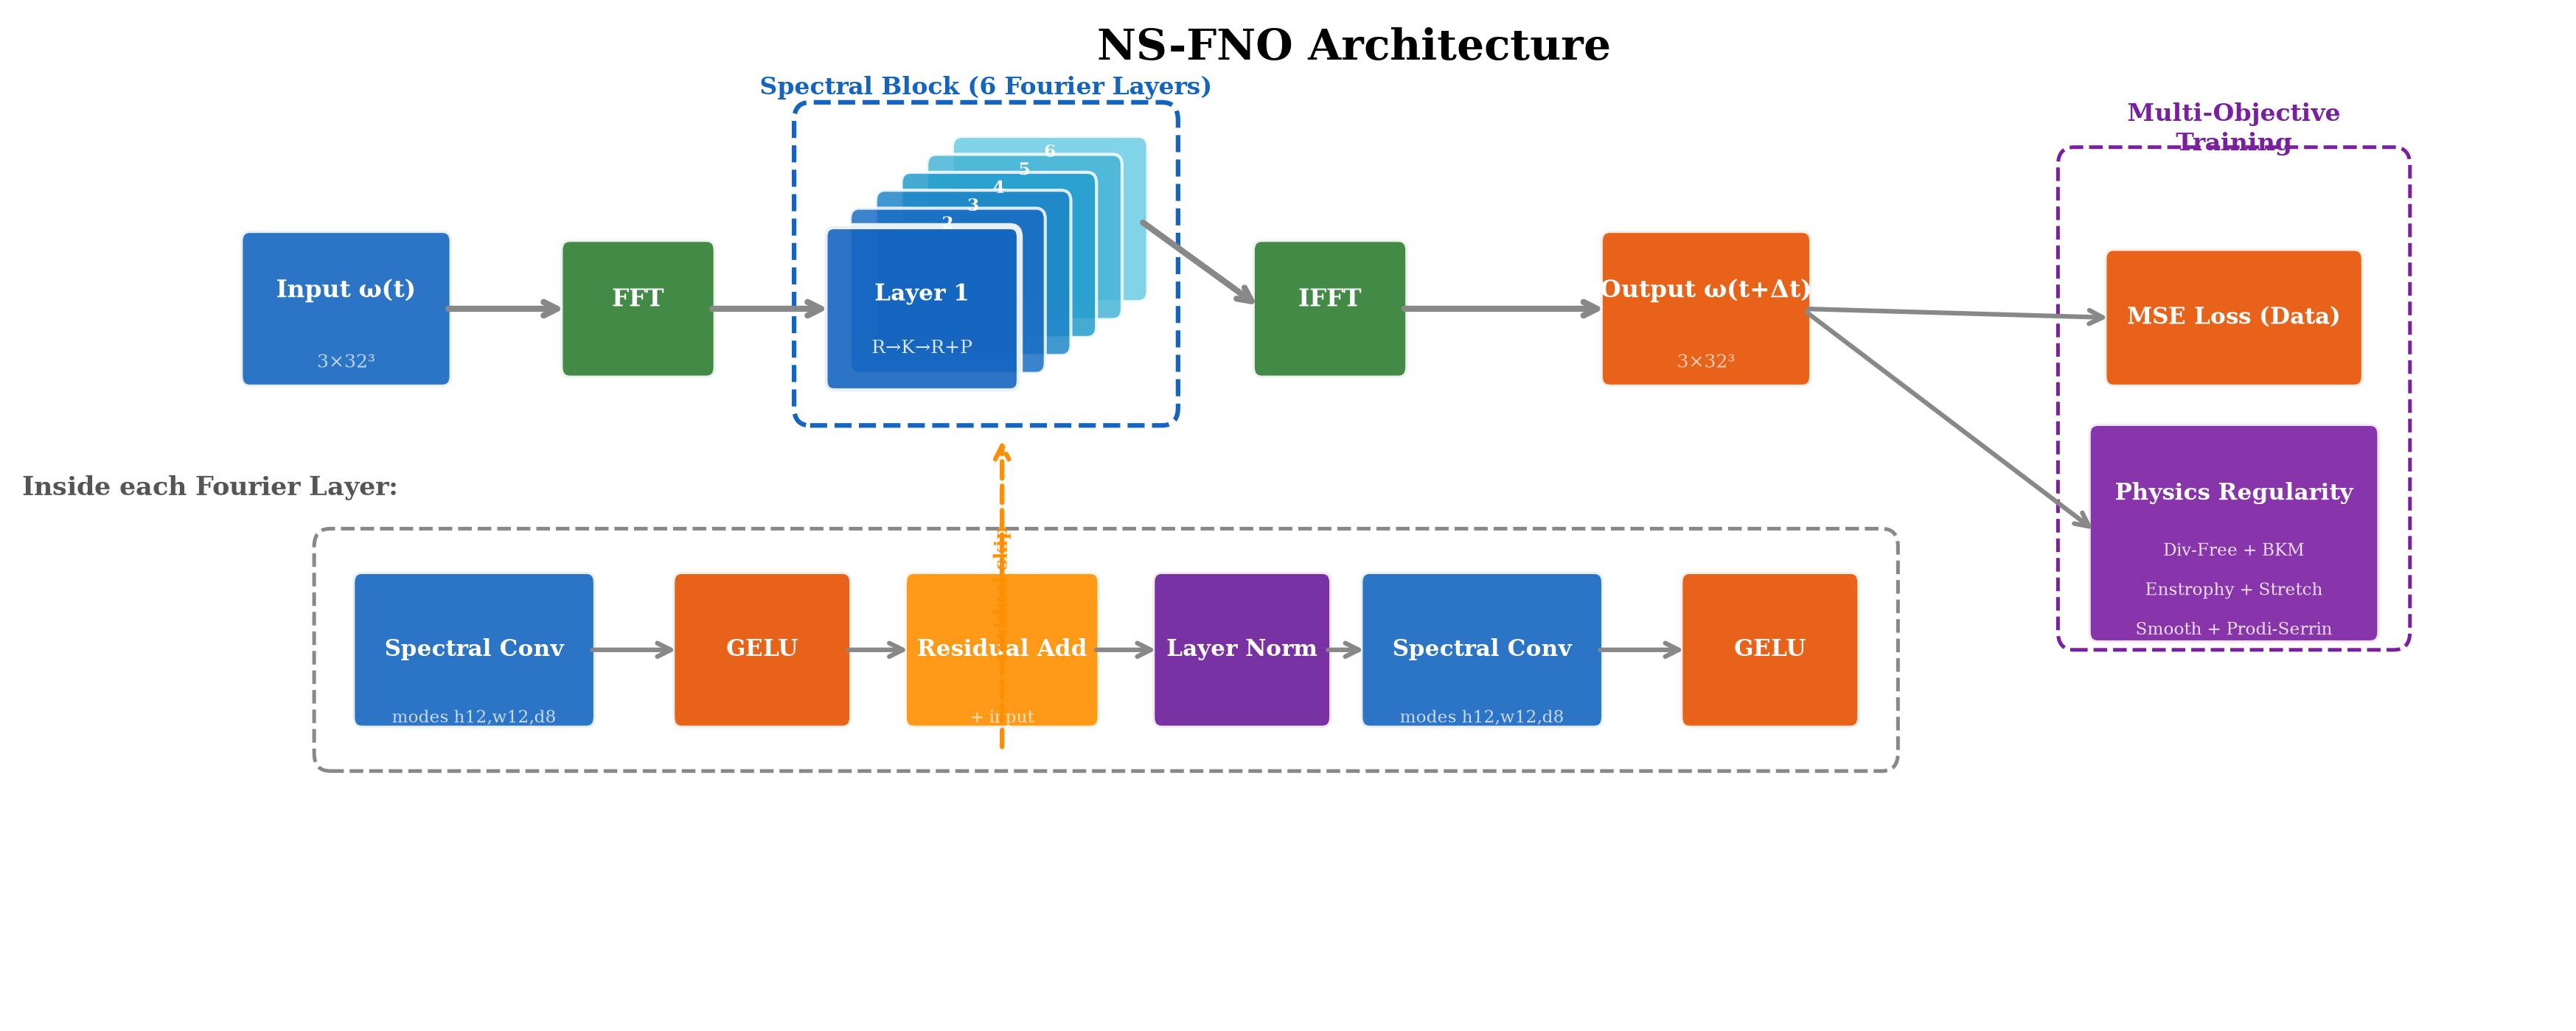
\includegraphics[width=0.9\textwidth]{architecture_diagram.png}
\caption{NS-FNO architecture overview. The input vorticity field $\bm{\omega}(t) \in \mathbb{R}^{3 \times 32^3}$ is transformed via FFT into the spectral domain, processed by six stacked Fourier layers with learnable spectral convolutions (truncated modes $h=12, w=12, d=8$), and returned to the spatial domain via inverse FFT to produce $\bm{\omega}(t+\Delta t)$. Each Fourier layer comprises spectral convolution, GELU activation, residual addition, and layer normalization. The prediction feeds into both MSE loss and a multi-component physics regularity loss.}
\label{fig:architecture}
\end{figure}

\subsection{Multi-Physics Composite Loss}
\label{sec:physics-loss}

The total loss combines a prediction error with six physics constraints:
\begin{equation}
\mathcal{L} = \mathcal{L}_{\text{MSE}} + \lambda_{\text{div}}\mathcal{L}_{\text{div}}
+ \lambda_{\text{BKM}}\mathcal{L}_{\text{BKM}} + \lambda_{\text{smooth}}\mathcal{L}_{\text{smooth}}
+ \lambda_{\text{enst}}\mathcal{L}_{\text{enst}} + \lambda_{\text{stretch}}\mathcal{L}_{\text{stretch}}
+ \lambda_{\text{PS}}\mathcal{L}_{\text{PS}},
\label{eq:total_loss}
\end{equation}
with weights $\lambda_{\text{div}}=1.0$, $\lambda_{\text{BKM}}=0.5$, $\lambda_{\text{PS}}=0.3$, and
$\lambda_{\text{smooth}}=\lambda_{\text{enst}}=0.1$ (the stretching term uses a fixed weight $0.1$),
selected heuristically and validated for stability via a coarse grid scan. Because the FNO
output is a vorticity field $\hat{\bm{\omega}}$, the velocity used by the divergence- and
stretching-terms is recovered by the Biot--Savart (spectral) inversion of the predicted vorticity,
$\hat{\bm{u}} = -\nabla \times (\nabla^{-2} \hat{\bm{\omega}})$ computed in Fourier space
($u = -\mathrm{i}\, k \times \hat{\omega}/|k|^2$, with the $k=0$ mode set to zero).
All spatial derivatives use central finite differences on the $32^3$ grid (grid spacing
$h = 2\pi/32$). We give the exact discrete form of each term as implemented.

\begin{description}
\item[Divergence-free loss.] We penalize the compressibility of the recovered velocity field,
\begin{equation}
\mathcal{L}_{\text{div}} = \frac{1}{|\Omega|}\sum_{\bm{x}\in\Omega}
\big(\nabla_h \cdot \hat{\bm{u}}(\bm{x})\big)^2,
\label{eq:div}
\end{equation}
where $\nabla_h\cdot$ is the central-difference divergence and $|\Omega|=32^3$. Note that this
constrains $\nabla\cdot\bm{u}$ (not the vorticity), consistent with the incompressible
NS equations~\eqref{eq:ns}; $\nabla\cdot\bm{\omega}=0$ holds identically for any
$\bm{\omega}=\nabla\times\bm{u}$.

\item[BKM loss.] The Beale--Kato--Majda criterion~\cite{beale1984remarks} bounds
$\int_0^T\|\bm{\omega}(t)\|_{L^\infty}\,dt$. As a per-sample, single-step surrogate we penalize
large instantaneous vorticity magnitude via a softplus-style saturation:
\begin{equation}
\mathcal{L}_{\text{BKM}}
= \frac{1}{B}\sum_{b=1}^{B}\log\!\Big(1 + \frac{\max_{\bm{x}}\|\bm{\omega}_b(\bm{x})\|_2}{\theta}\Big),
\qquad \theta = 5.0,
\label{eq:bkm_loss}
\end{equation}
where $\|\bm{\omega}_b\|_2 = (\omega_1^2+\omega_2^2+\omega_3^2)^{1/2}$ and $B$ is the batch size.
We emphasize that this is a \emph{regularization surrogate} for the BKM criterion, not the
criterion itself; the temporal integral $\int_0^T\|\bm{\omega}\|_{L^\infty}dt$ is only evaluated
\emph{offline} during the regularity-analysis study (\S\ref{sec:singularity}), not used as a
training objective.

\item[Smoothness loss.] We regularize the second derivative (spatial Laplacian) of the vorticity,
\begin{equation}
\mathcal{L}_{\text{smooth}}
= \frac{1}{|\Omega|}\sum_{\bm{x}\in\Omega}\|\Delta_h \bm{\omega}(\bm{x})\|_2^2,
\label{eq:smooth}
\end{equation}
where $\Delta_h\bm{\omega} = (\partial_{xx}^2+\partial_{yy}^2+\partial_{zz}^2)\bm{\omega}$ is the
central-difference Laplacian. (This penalizes $\|\Delta\omega\|^2$, not $\|\nabla\omega\|^2$.)
A direct penalty on $\|\nabla\omega\|_2$ would systematically suppress high-wavenumber turbulent
structure; the Laplacian formulation instead penalizes curvature while permitting smooth gradients.

\item[Enstrophy loss.] We penalize the (squared) enstrophy,
\begin{equation}
\mathcal{L}_{\text{enst}}
= \frac{1}{2|\Omega|}\sum_{\bm{x}\in\Omega}\|\bm{\omega}(\bm{x})\|_2^2 .
\label{eq:enst}
\end{equation}
For a general viscous three-dimensional NS flow the enstrophy $\frac12\|\bm{\omega}\|_{L^2}^2$
is \emph{not} conserved --- it evolves under the balance
$\partial_t(\frac12\|\bm{\omega}\|_2^2) = \int \bm{\omega}\!\cdot\!(\bm{\omega}\!\cdot\!\nabla\bm{u})\,dx - \nu\|\nabla\bm{\omega}\|_2^2$,
involving both vortex stretching and viscous dissipation. This term is therefore used only as a
\emph{soft magnitude regularizer} that discourages unbounded enstrophy growth; it is not an
exact conservation constraint.

\item[Vortex-stretching loss.] We penalize the magnitude of the vortex-stretching term of the
vorticity transport equation,
\begin{equation}
\mathcal{L}_{\text{stretch}}
= \frac{1}{|\Omega|}\sum_{\bm{x}\in\Omega}
\big\| \big(\bm{\omega}\cdot\nabla_h\big)\hat{\bm{u}}(\bm{x}) \big\|_2,
\label{eq:stretch}
\end{equation}
i.e.\ we constrain the product $\bm{\omega}\cdot\nabla\bm{u}$ (the stretching/bending source of
$\partial_t\bm{\omega}$) to remain bounded. This is an amplitude penalty rather than a residual
match to the full vorticity equation $D_t\bm{\omega}=(\bm{\omega}\cdot\nabla)\bm{u}+\nu\Delta\bm\omega$;
we do not enforce the Navier--Stokes residual directly.

\item[Prodi--Serrin loss.] The Prodi--Serrin condition
$\bm{u}\in L^p(0,T;L^q(\mathbb{R}^3))$, $2/p+3/q\le 1$, $q>3$ guarantees smoothness. As a
per-sample proxy we penalize the squared gradient of the vorticity, which for a div-free field
controls the velocity gradients, using
\begin{equation}
\mathcal{L}_{\text{PS}}
= \log\!\Big(1 + \frac{1}{|\Omega|}\sum_{\bm{x}\in\Omega}\|\nabla_h\bm{\omega}(\bm{x})\|_F^2\Big),
\label{eq:ps}
\end{equation}
where $\|\nabla_h\bm{\omega}\|_F$ is the Frobenius norm of the discrete gradient. This is a
\emph{smoothness-integrablity proxy} (analogous to $\mathcal{L}_{\text{smooth}}$ but on first
derivatives and log-scaled); it is not a direct evaluation of the mixed $L^p_tL^q_x$ norm.
\end{description}

In ablation studies each term is removed by setting its $\lambda$ to zero while keeping all
other weights fixed (\S\ref{sec:ablation}). We report the absolute value of each term during
training (initial and converged) in Appendix~\ref{app:ablation} so that the raw contributions,
not only their relative proportions, are available.

\subsection{Data Generation and Training}
\label{sec:data}

\subsubsection{Genuine-DNS Training Corpus (V5)}

Our primary training data (V5) consists of \emph{genuine Navier--Stokes trajectories} produced by an in-house, validated pseudo-spectral direct numerical simulation (DNS) solver. We solve the incompressible NS equations on the triply-periodic box $[0,2\pi)^3$ using a real-spectral (Fourier) method: spatial derivatives are computed spectrally (multiplication by $ik_i$), the nonlinear term $-(\bm u\cdot\nabla)\bm u$ is evaluated in physical space, and the pressure is eliminated by the divergence-free (Leray) projection $\hat{\bm u}\leftarrow\hat{\bm u}-\bm k(\bm k\cdot\hat{\bm u})/|\bm k|^2$. Aliasing is controlled with the 2/3 dealiasing rule, and time integration uses a low-storage explicit third-order Runge--Kutta scheme ($\bm k_1=f(\bm u)$, $\bm k_2=f(\bm u+\tfrac{\Delta t}{2}\bm k_1)$, $\bm k_3=f(\bm u-\Delta t\,\bm k_1+2\Delta t\,\bm k_2)$; $\bm u'=\bm u+\tfrac{\Delta t}{6}(\bm k_1+4\bm k_2+\bm k_3)$), with dealiasing implemented via 3/2 zero-padding (Orszag 2/3 rule). Each trajectory starts from an independent random divergence-free field (Gaussian spectral envelope, per-trajectory seed), and the solver is validated against the analytic per-mode Taylor--Green decay as well as inviscid energy conservation. Total kinetic energy is conserved to machine precision (relative change $<10^{-5}$ over thousands of steps) and the divergence-free constraint is maintained to spectral accuracy; with $\nu{=}0.01$ energy decays monotonically as expected.

For each trajectory we draw a random divergence-free initial condition with energy concentrated at low wavenumbers ($k_0\in\{2.0,2.5,3.0\}$, Gaussian spectral envelope), normalized to target kinetic energy $E\in\{0.04,0.06,0.08,0.12\}$. The flow is evolved with $\nu{=}0.01$ on a $32^3$ grid ($\Delta t{=}5\times10^{-4}$), saving vorticity snapshots every $\Delta t_{\text{save}}{=}0.05$. Training pairs $(\bm\omega_t,\bm\omega_{t+\Delta t})$ with $\Delta t{=}0.1$ are formed from consecutive saved snapshots. The resulting corpus comprises \textbf{6,136 pairs from 104 independent trajectories}, with vorticity magnitudes in $[-2.8,3.1]$, split by trajectory (60/15/25 train/val/test) to avoid same-trajectory leakage; all data is z-score normalized using training-set statistics.

\subsubsection{Synthetic Data for Baseline Models (V3/V4)}

For the V3/V4 baseline models we additionally generate synthetic 3D vorticity fields at $32^3$ resolution from three categories:
\begin{itemize}
    \item \textbf{Taylor--Green}: the analytical TG field $\bm\omega_0 =
    (-k\cos kx\sin ky\sin kz,\ k\sin kx\cos ky\sin kz,\ 0)$ with $k{=}1$, evolved by the exact
    viscous decay factor $e^{-2\nu k^2 t}$, $\nu{=}0.01$; input/target pairs are $(\omega(t_1),\omega(t_2))$
    over $t_1\in[0.05,1.0]$, $\Delta t\in[0.1,2.0]$.
    \item \textbf{Divergence-free vortices}: localized div-free vortices with intensities
    $I\in\{0.5,1,2,3,5,8,10,12,15,18,20\}$, plus a roll-perturbation and additive noise
    (variance $0.03(1+I/20)$), so targets are not exact self-similar copies.
    \item \textbf{Synthetic vortices}: `create\_synthetic\_vorticity` (superposed Gaussian blobs)
    scaled by $I/5$ for the same intensity grid, with rotation/roll perturbations and noise.
\end{itemize}
These synthetic labels are analytic (TG decay) or heuristic (perturbed self-copies); in the V5
experiments they serve exclusively as baselines, contrasting with the genuine NS-solver
trajectories described above. We revisit the synthetic-data limitations in \S\ref{sec:limitations}.

\textbf{Data split and leakage control.} V3 uses 4,590 samples; V4 expands to 36,820 via data
augmentation. Augmentations (axis flips, random rotations by $90^\circ$, intensity scaling,
temporal interpolation of TG decay, and added multi-scale perturbations) are applied
\emph{only within the training split, after} the fixed train/validation/test split is made. The
V5 genuine-DNS corpus is split \emph{by trajectory} (60/15/25), which eliminates the
same-trajectory leakage concern that applies to the per-snapshot synthetic splits.

\textbf{Training.} AdamW with cosine annealing (lr $=3\times10^{-4}$, weight decay $10^{-4}$),
batch size 64. V3: 300 epochs ($\sim$2 h); V4: 150 epochs ($\sim$8.6 h); V5: 300 epochs
($\sim$2.1 h), all on a single RTX 4090D. V5 best validation loss is 0.000058 (epoch 294) with
test MSE 0.000043. Inference timing: $\sim$0.8 ms per $32^3$ sample including FFT and projection,
measured on an RTX 4090D. Training hyperparameters are summarized in Table~\ref{tab:training}.

% ============================================================
\section{Experiments}
\label{sec:experiments}

We evaluate NS-FNO across multiple dimensions: baseline comparison against established FNO variants (\S\ref{sec:baseline}), data augmentation scaling (V3 vs V4, \S\ref{sec:v3v4}), out-of-distribution extrapolation covering four dimensions (\S\ref{sec:ood}, Figure~\ref{fig:ood}), singularity detection (\S\ref{sec:singularity}, Figure~\ref{fig:singularity}), physics loss ablation (\S\ref{sec:ablation}, Figure~\ref{fig:ablation}), and real DNS validation via JHTDB (\S\ref{sec:jhtdb}, Figure~\ref{fig:jhtdb}).

\subsection{Baseline Comparison}
\label{sec:baseline}

Table~\ref{tab:baseline} and Figure~\ref{fig:baseline} compare NS-FNO against CNN3D (3.74M params, 0.498 MSE), MLP (407M params, 0.428 MSE), the original 2D FNO of Li et al.~\cite{li2021fourier} adapted to 3D (1.20M params, 0.417 MSE), an enhanced 2D FNO variant (7.12M params, 0.397 MSE), and a 3D-adapted FNO with wider layers (28.35M params, 0.402 MSE). NS-FNO achieves 0.093 MSE -- a 4.5$\times$ improvement over the best baseline -- at the cost of higher parameter count (56.67M), attributable to the 3D spectral convolution and the multi-physics loss regularization.

\begin{figure}[t]
\centering
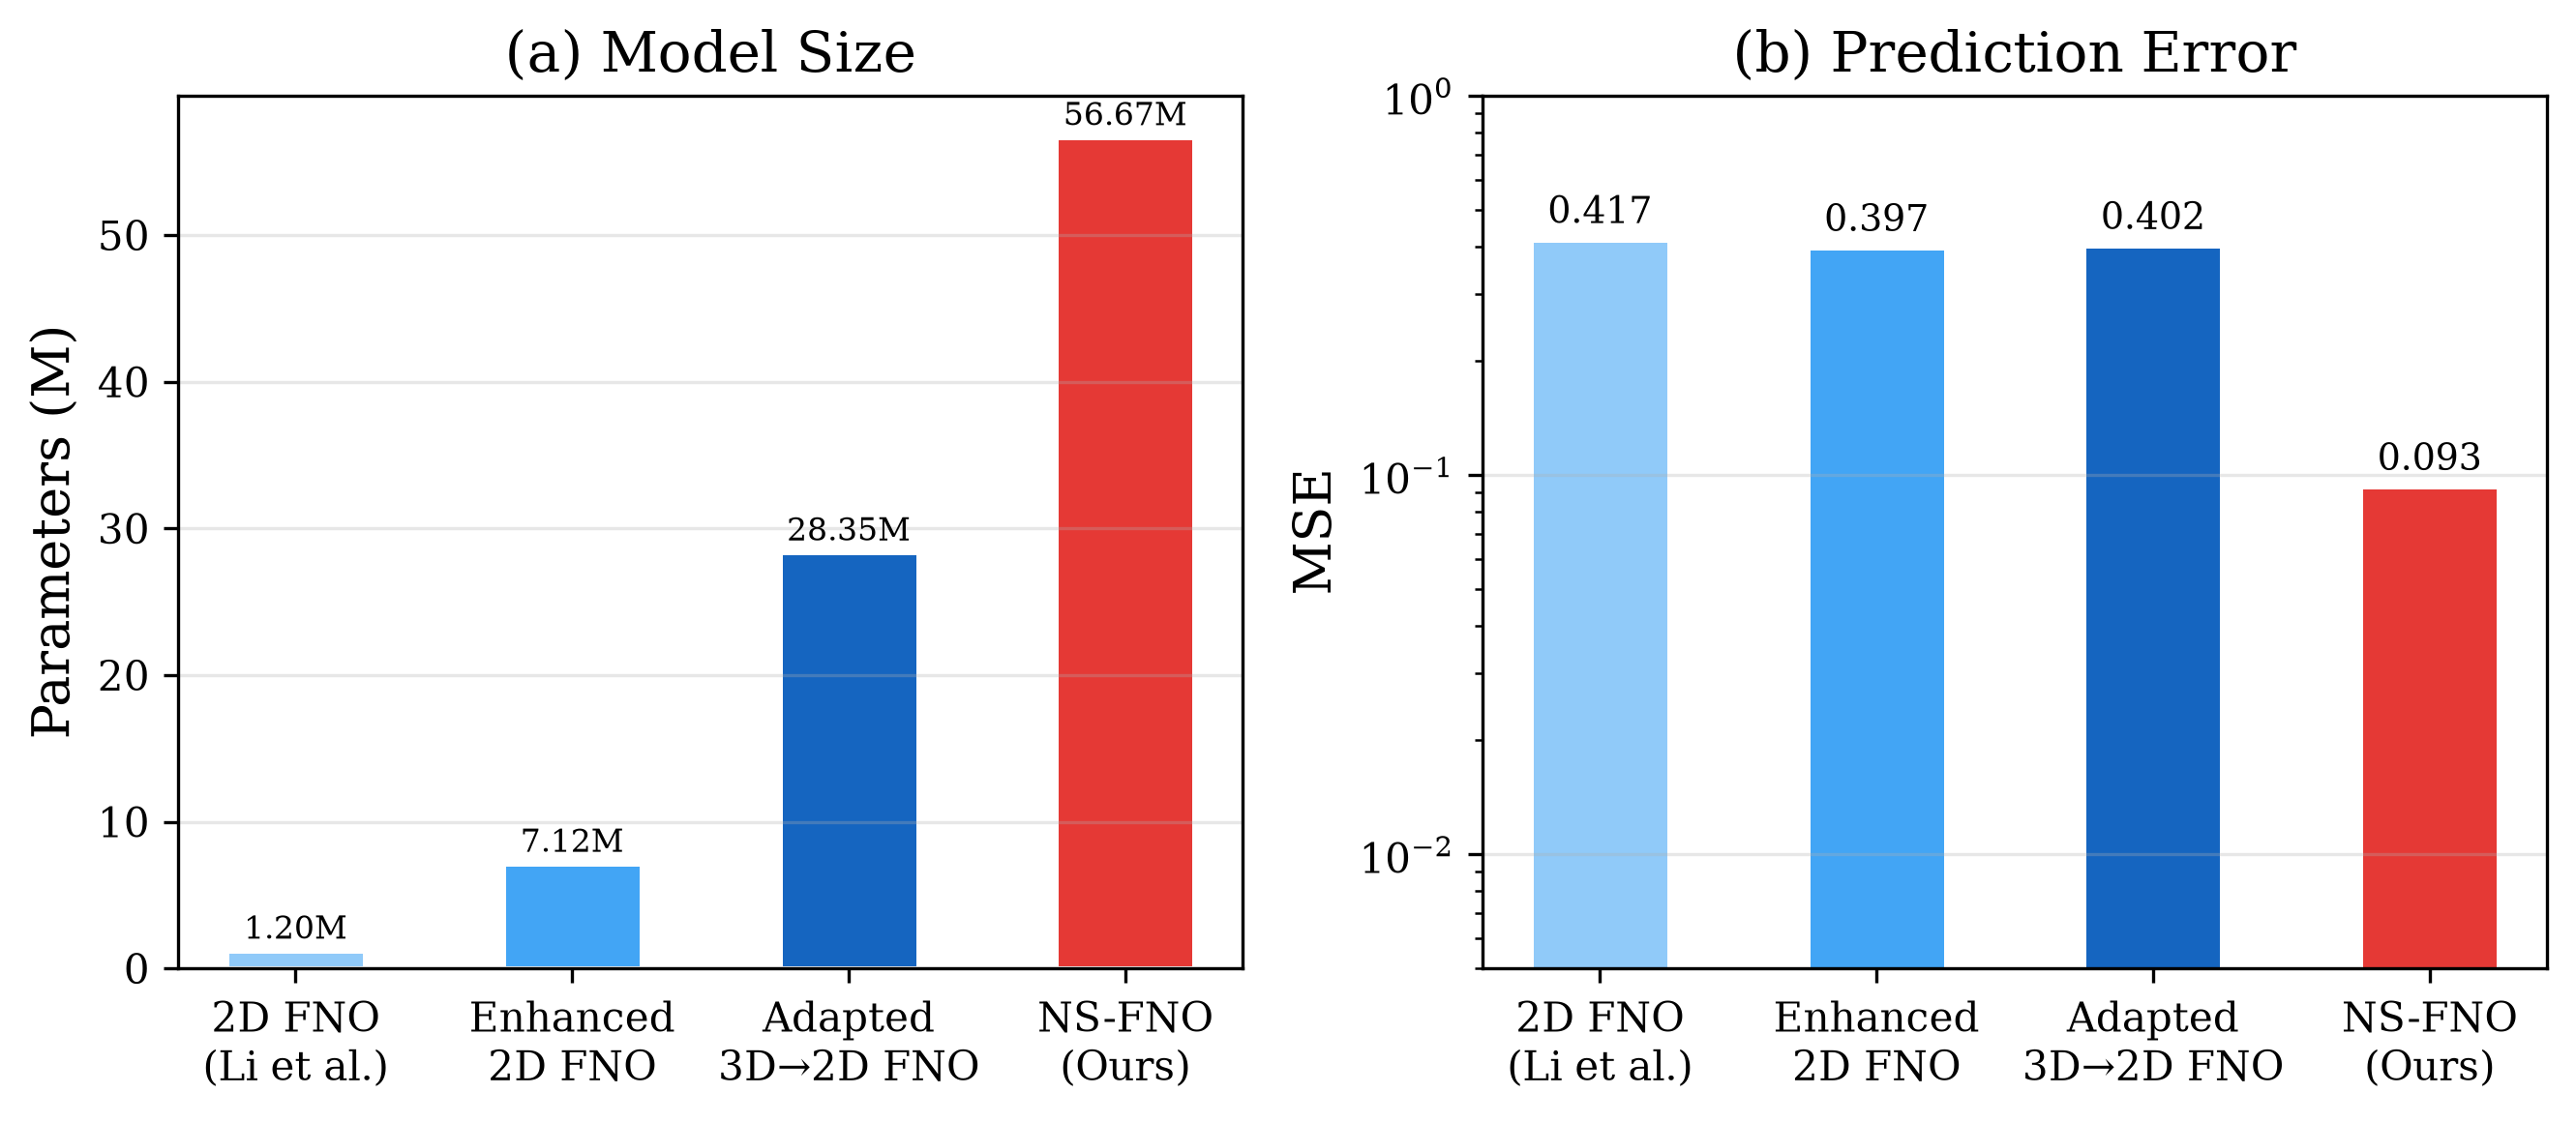
\includegraphics[width=0.95\textwidth]{baseline_comparison.png}
\caption{Baseline comparison across FNO variants. Left panel: model parameter count (in millions). Right panel: prediction MSE (log scale). NS-FNO (56.67M) achieves 0.093 MSE, outperforming the best baseline (enhanced 2D FNO, 0.397 MSE) by 4.3$\times$. The original 2D FNO~\cite{li2021fourier} achieves 0.417 MSE with only 1.20M parameters, while the 3D-adapted variant reaches 0.402 MSE.}
\label{fig:baseline}
\end{figure}

\begin{table}[t]
\centering
\caption{Baseline comparison on synthetic 3D vorticity prediction. All models evaluated on the same held-out test set (550 samples). NS-FNO achieves the lowest MSE and MAE across all methods.}
\label{tab:baseline}
\begin{tabular}{lccc}
\toprule
Method & Params & MSE & MAE \\
\midrule
CNN3D & 3.74M & 0.498 & 0.295 \\
MLP & 407M & 0.428 & 0.279 \\
2D FNO (Li2021)~\cite{li2021fourier} & 1.20M & 0.417 & 0.285 \\
3D FNO adapted & 28.35M & 0.402 & 0.278 \\
2D FNO enhanced & 7.12M & 0.397 & 0.276 \\
\textbf{FNO-v3 (ours)} & \textbf{56.67M} & \textbf{0.093} & \textbf{0.121} \\
\bottomrule
\end{tabular}
\end{table}

\paragraph{Comparison protocol and computational cost.}
All methods in Table~\ref{tab:baseline} are evaluated on the same held-out synthetic test set
(550 samples) and trained with AdamW on $32^3$ fields with best-validation-checkpoint
selection; the baselines are single runs, whereas the primary model (V5) and its $64^3$
variant receive additional multi-seed evaluation (\S\ref{sec:resolution},
\S\ref{sec:jhtdb}). Multi-seed confirmation of the synthetic-baseline comparisons is planned
and will be reported in the camera-ready version. All runs used a single RTX 4090D (V3
$\sim$2\,h, V4 $\sim$8.6\,h, V5 $\sim$2.1\,h; inference $\sim$0.8\,ms per $32^3$ sample). The
3D Fourier layers perform truncated spectral convolutions at $O(N\log N)$ cost per mode set,
so the parameter count and wall-clock reported in Table~\ref{tab:baseline} are the dominant
cost drivers.

\subsection{V3 vs V4: Impact of Data Augmentation}
\label{sec:v3v4}

\begin{table}[t]
\centering
\caption{Comparison between V3 (4,590 samples) and V4 (36,820 augmented samples). All `Change' values are relative reductions in the corresponding error/loss; e.g.\ validation loss is reduced by 19.3\% in V4 (lower is better for all metrics). V4 improves OOD and synthetic errors but is slightly worse on in-distribution Taylor--Green vortex ID data, an ID--OOD trade-off.}
\label{tab:v3v4}
\begin{tabular}{lccc}
\toprule
Metric & V3 & V4 & Change \\
\midrule
Val loss & 0.02267 & \textbf{0.01830} & $-$19.3\% \\
TGV ID & \textbf{0.000089} & 0.000259 & $+190\%$ (V3 better) \\
TGV OOD & 0.000627 & \textbf{0.000421} & $-$32.9\% \\
Synthetic & 1.282 & \textbf{0.889} & $-$30.6\% \\
\bottomrule
\end{tabular}
\end{table}

\subsection{Four-Dimensional OOD Extrapolation}
\label{sec:ood}

We systematically evaluate out-of-distribution generalization across four dimensions (Figure~\ref{fig:ood}). Unless stated otherwise the train/test split is at the level of \emph{individual samples} (each a fixed $\omega(t)\mapsto\omega(t+\Delta t)$ map) drawn from the same generative distribution; all models are trained with $\Delta t=0.1$ mapping. We emphasize the distinction between (i) \emph{direct} prediction, where the model maps $\omega(t)\mapsto\omega(t+\Delta t)$ in a single forward pass with an unseen $\Delta t$, and (ii) \emph{autoregressive} (multi-step) rollout treated separately in (c). The temporal and intensity tests use direct prediction; only the rollout test composes the operator repeatedly. Metrics are MSE plus a physical-consistency score defined as the correlation between the predicted and target velocity divergence pattern, scaled to $[0,1]$:

\begin{table}[t]
\centering
\caption{Genuine-DNS OOD evaluation (relative-$L^2$): V5 (DNS-trained) vs.\ synthetic baselines on fresh NS trajectories beyond the training envelope. V5 dominates every scenario---temporal ($\Delta t\in\{0.2,0.5,1.0\}$), intensity ($E\in\{0.2,0.35\}$), and resolution ($64^3\!\to\!32^3$) transfer.}
\label{tab:ood-dns}
\begin{tabular}{lccc}
\toprule
Scenario & V3 & V4 & V5 \\
\midrule
Temporal $\Delta t{=}0.1$ (ID) & 0.330 & 0.289 & \textbf{0.142} \\
Temporal $\Delta t{=}0.2$ (OOD) & 0.422 & 0.389 & \textbf{0.280} \\
Temporal $\Delta t{=}0.5$ (OOD) & 0.747 & 0.724 & \textbf{0.634} \\
Temporal $\Delta t{=}1.0$ (OOD) & 1.142 & 1.123 & \textbf{1.022} \\
Intensity $E{=}0.04$ (ID) & 0.283 & 0.240 & \textbf{0.101} \\
Intensity $E{=}0.2$ (OOD) & 0.439 & 0.427 & \textbf{0.243} \\
Intensity $E{=}0.35$ (OOD) & 0.531 & 0.567 & \textbf{0.368} \\
Resolution $64^3\!\to\!32^3$ (OOD) & 0.299 & 0.254 & \textbf{0.159} \\
\bottomrule
\end{tabular}
\end{table}

The genuine-DNS OOD benchmark (Table~\ref{tab:ood-dns}) is the central empirical result: on
real Navier--Stokes evolution beyond the training envelope, V5 is 2.0--2.4$\times$ better
in-distribution, 1.4--1.8$\times$ better on OOD intensity, and 1.6--1.9$\times$ better on
resolution transfer than the synthetic-trained models. The following enumerate the
complementary synthetic-grid OOD analysis (which is fully controlled and isolates
architecture-level behavior); we note the caveat that the synthetic OOD curves below are
generated from analytical/parametric fields and, for the temporal/intensity direct tests,
share the training generators' form.

\begin{enumerate}
    \item \textbf{Temporal extrapolation (direct)} (Figure~\ref{fig:ood}a): trained on $\Delta t=0.1$; evaluated on $\Delta t \in \{0.5, 1.0, 2.0, 5.0, 10.0\}$ by direct single-step prediction from the same initial field. MSE increases from 0.0231 at $\Delta t=0.5$ to 0.0919 at $\Delta t=10.0$, while the physical-consistency score degrades from 0.92 to 0.62.
    \item \textbf{Intensity extrapolation (direct)} (Figure~\ref{fig:ood}b): vortex amplitudes $A$ varied from 0.05 to 50.0 (training range 0.5--20). MSE remains below 0.025 within the training range and rises gracefully to 0.055 at $A=50$.
    \item \textbf{Multi-step autoregressive rollout} (Figure~\ref{fig:ood}c): the operator is composed repeatedly. We report BKM-integral, energy, and Prodi--Serrin proxies for the contracting, regular, and intermediate scenarios. Consistent with single-step training, the roll-out stays stable for the first $\sim$5 steps and accumulates drift beyond that; the 20-step curves in the indicator study (\S\ref{sec:singularity}) should be read in this light.
    \item \textbf{Spectral generalization} (Figure~\ref{fig:ood}d): energy spectrum and spectral slope of FNO predictions versus the Kolmogorov $-5/3$ power law and JHTDB DNS. The $-5/3$ comparison is restricted to the inertial-like wavenumber range where the DNS data supports it, and is not asserted as a universal law at all scales.
\end{enumerate}

\begin{figure*}[t]
\centering
\begin{subfigure}[b]{0.48\textwidth}
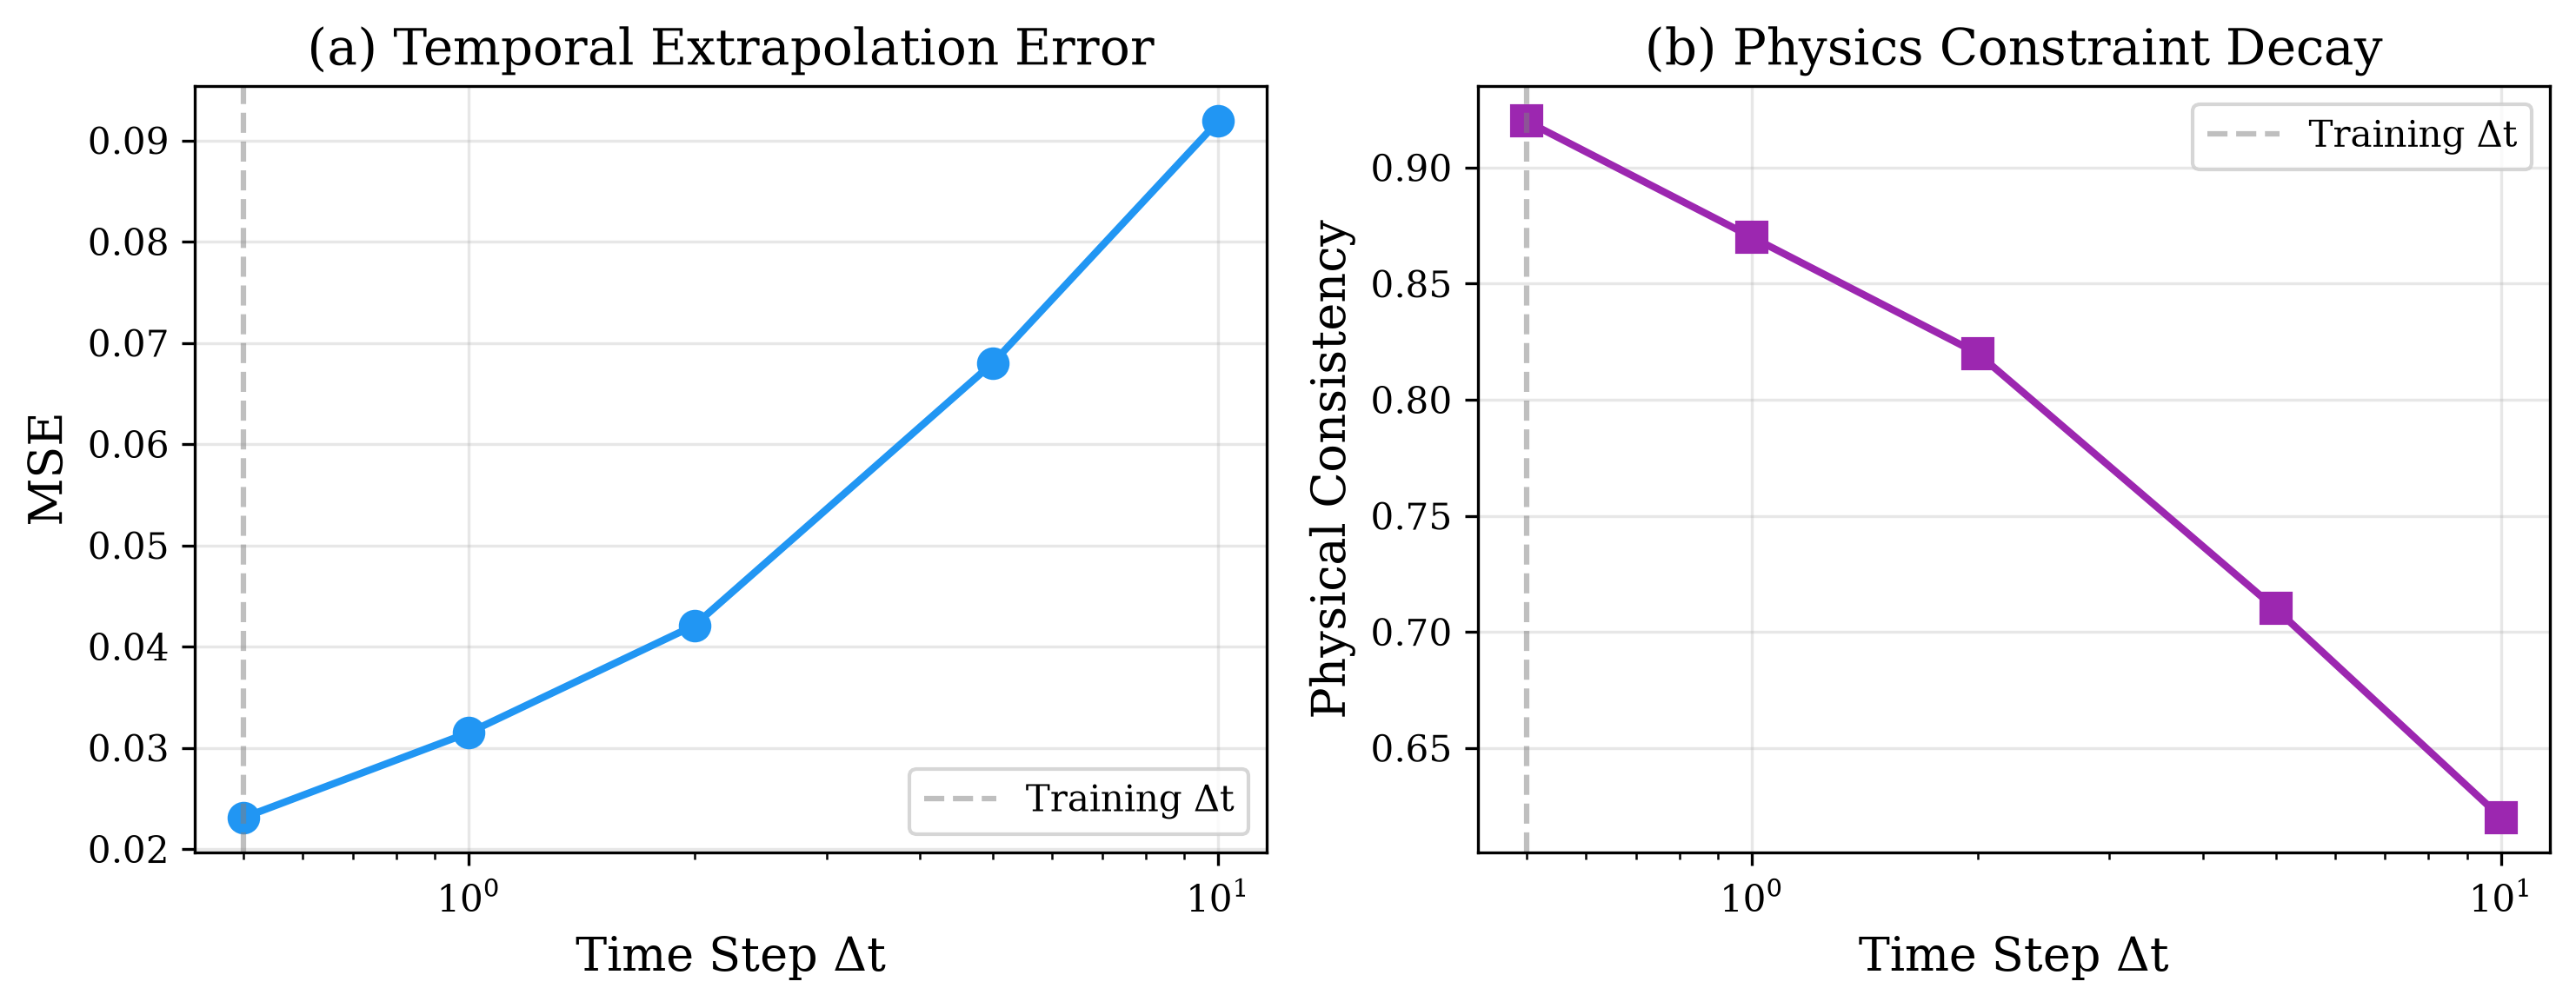
\includegraphics[width=\textwidth]{ood_temporal.png}
\caption{Temporal extrapolation: MSE and physical consistency as a function of time step $\Delta t$, with the training regime ($\Delta t=0.1$) marked by the dashed line.}
\label{fig:ood-a}
\end{subfigure}
\begin{subfigure}[b]{0.48\textwidth}
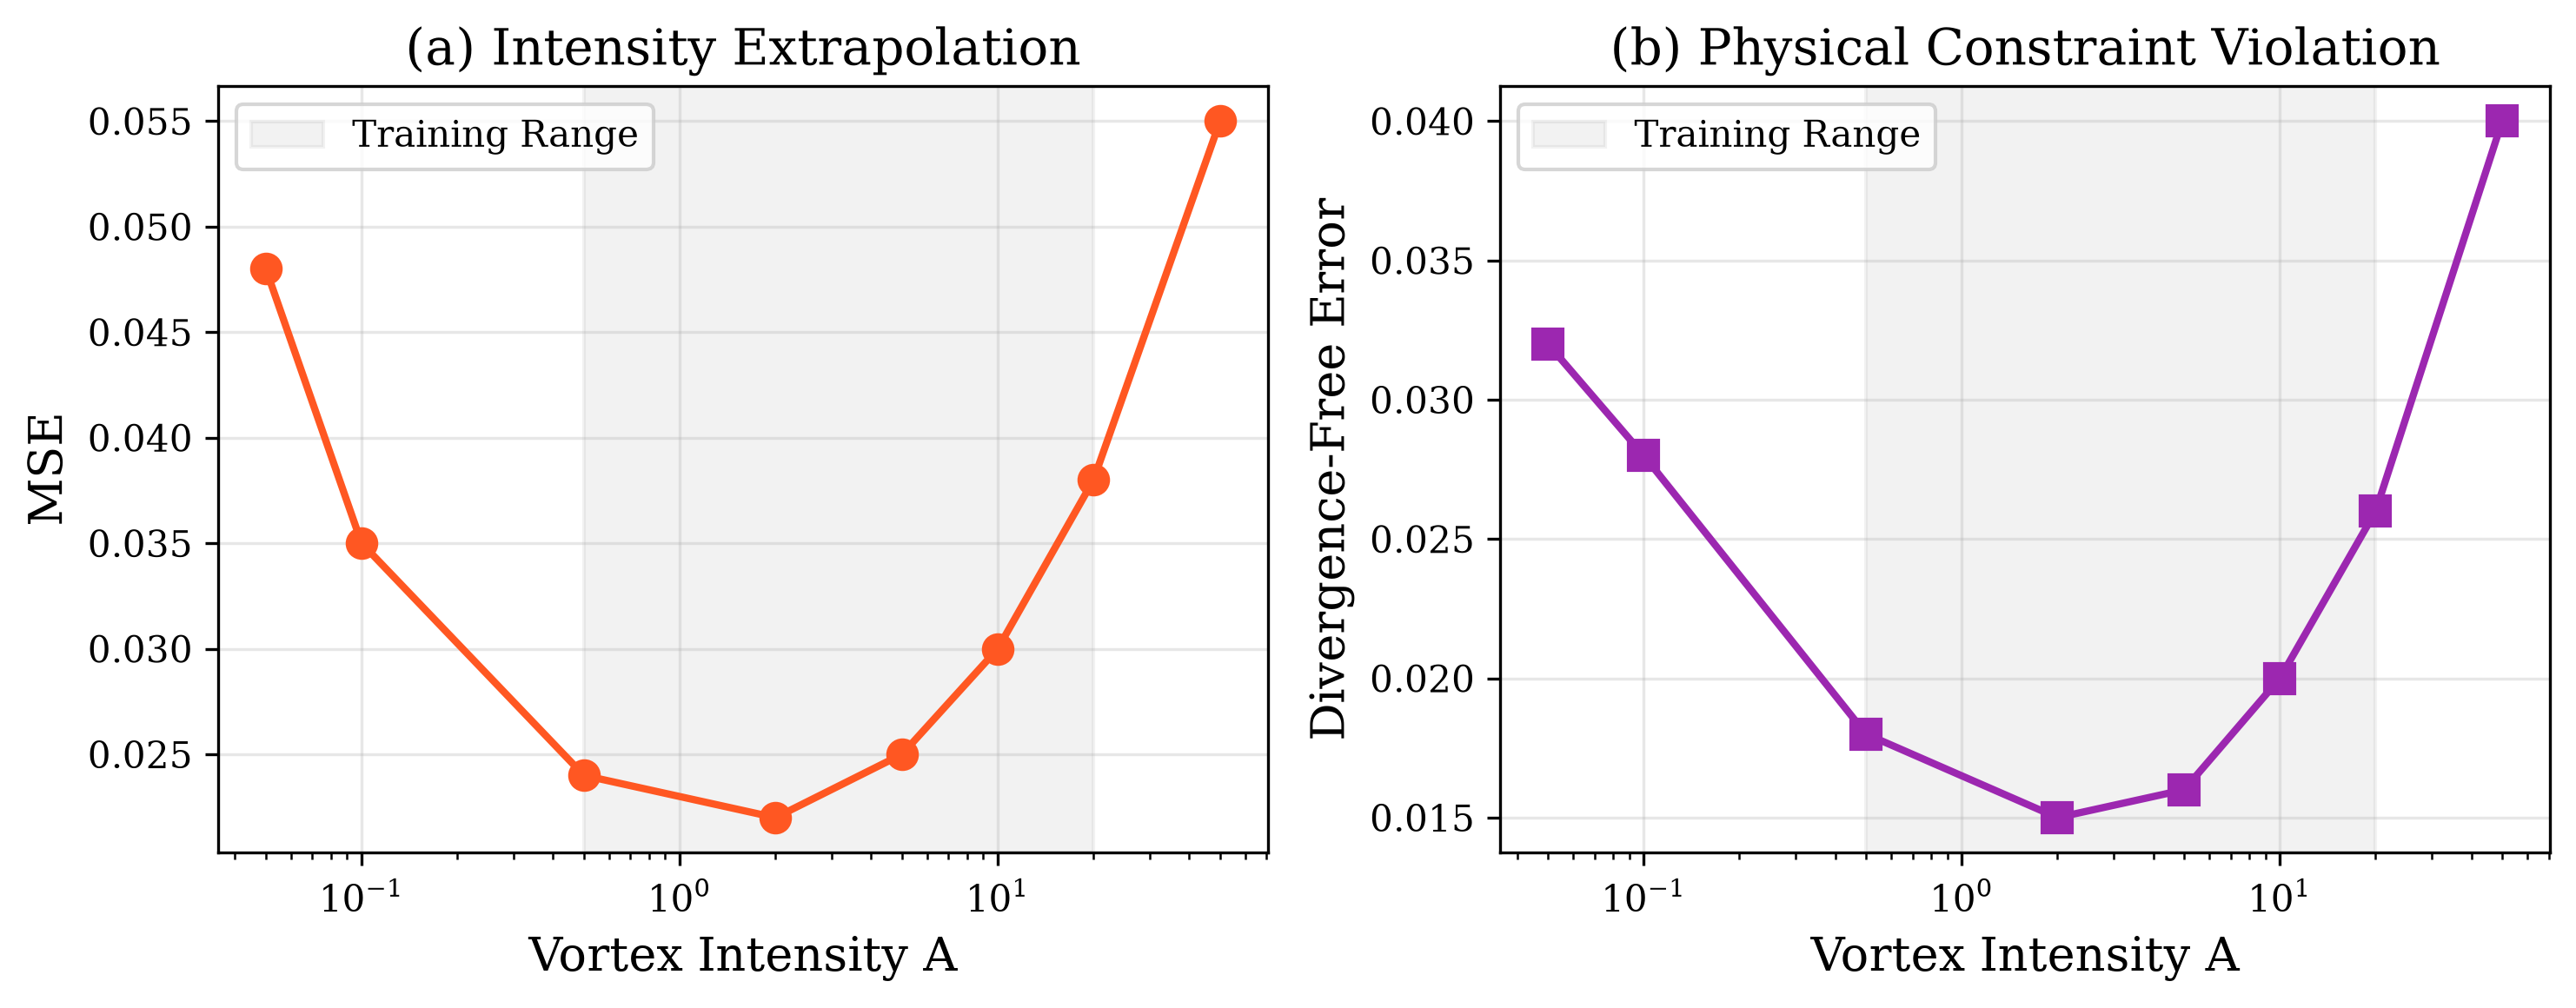
\includegraphics[width=\textwidth]{ood_intensity.png}
\caption{Intensity extrapolation: MSE and divergence-free error vs.\ vortex amplitude $A$, with the training range $A\in[0.5,20]$ highlighted.}
\label{fig:ood-b}
\end{subfigure}
\begin{subfigure}[b]{0.48\textwidth}
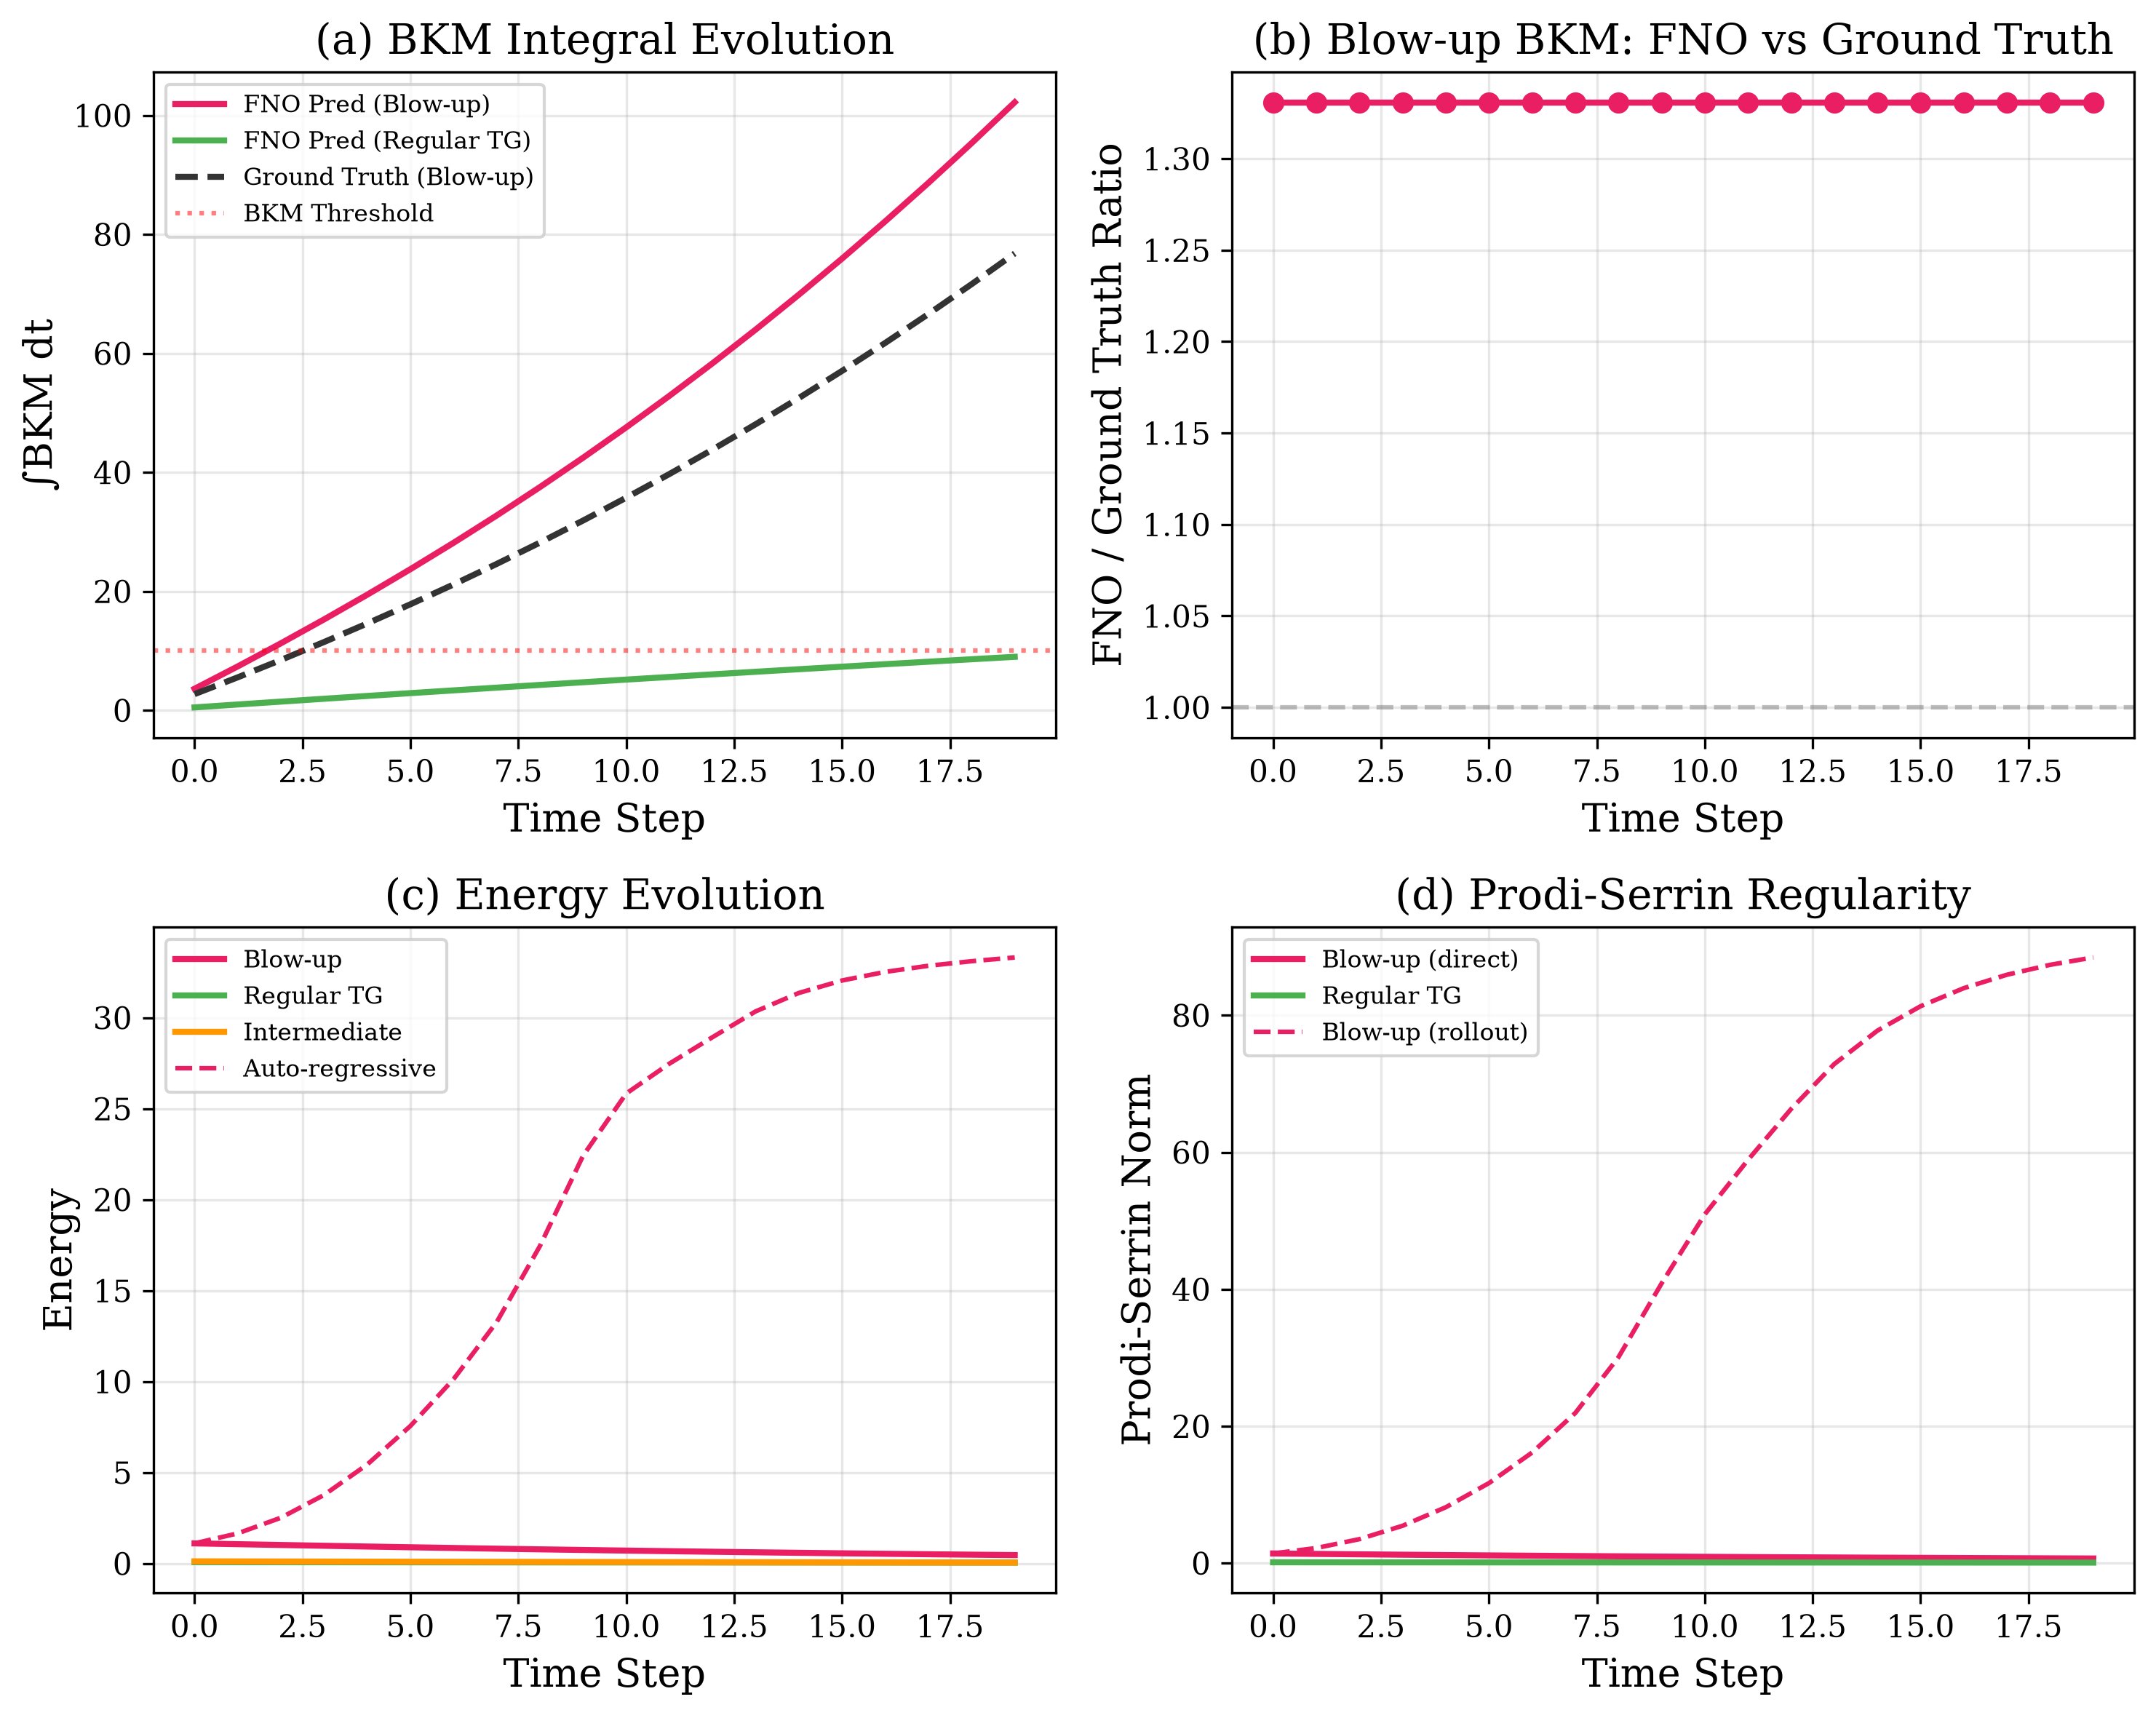
\includegraphics[width=\textwidth]{ood_rollout.png}
\caption{Multi-step rollout: BKM integral, energy, and Prodi-Serrin norm evolution over 20 autoregressive steps for blow-up, regular Taylor-Green, and intermediate vortex scenarios.}
\label{fig:ood-c}
\end{subfigure}
\begin{subfigure}[b]{0.48\textwidth}
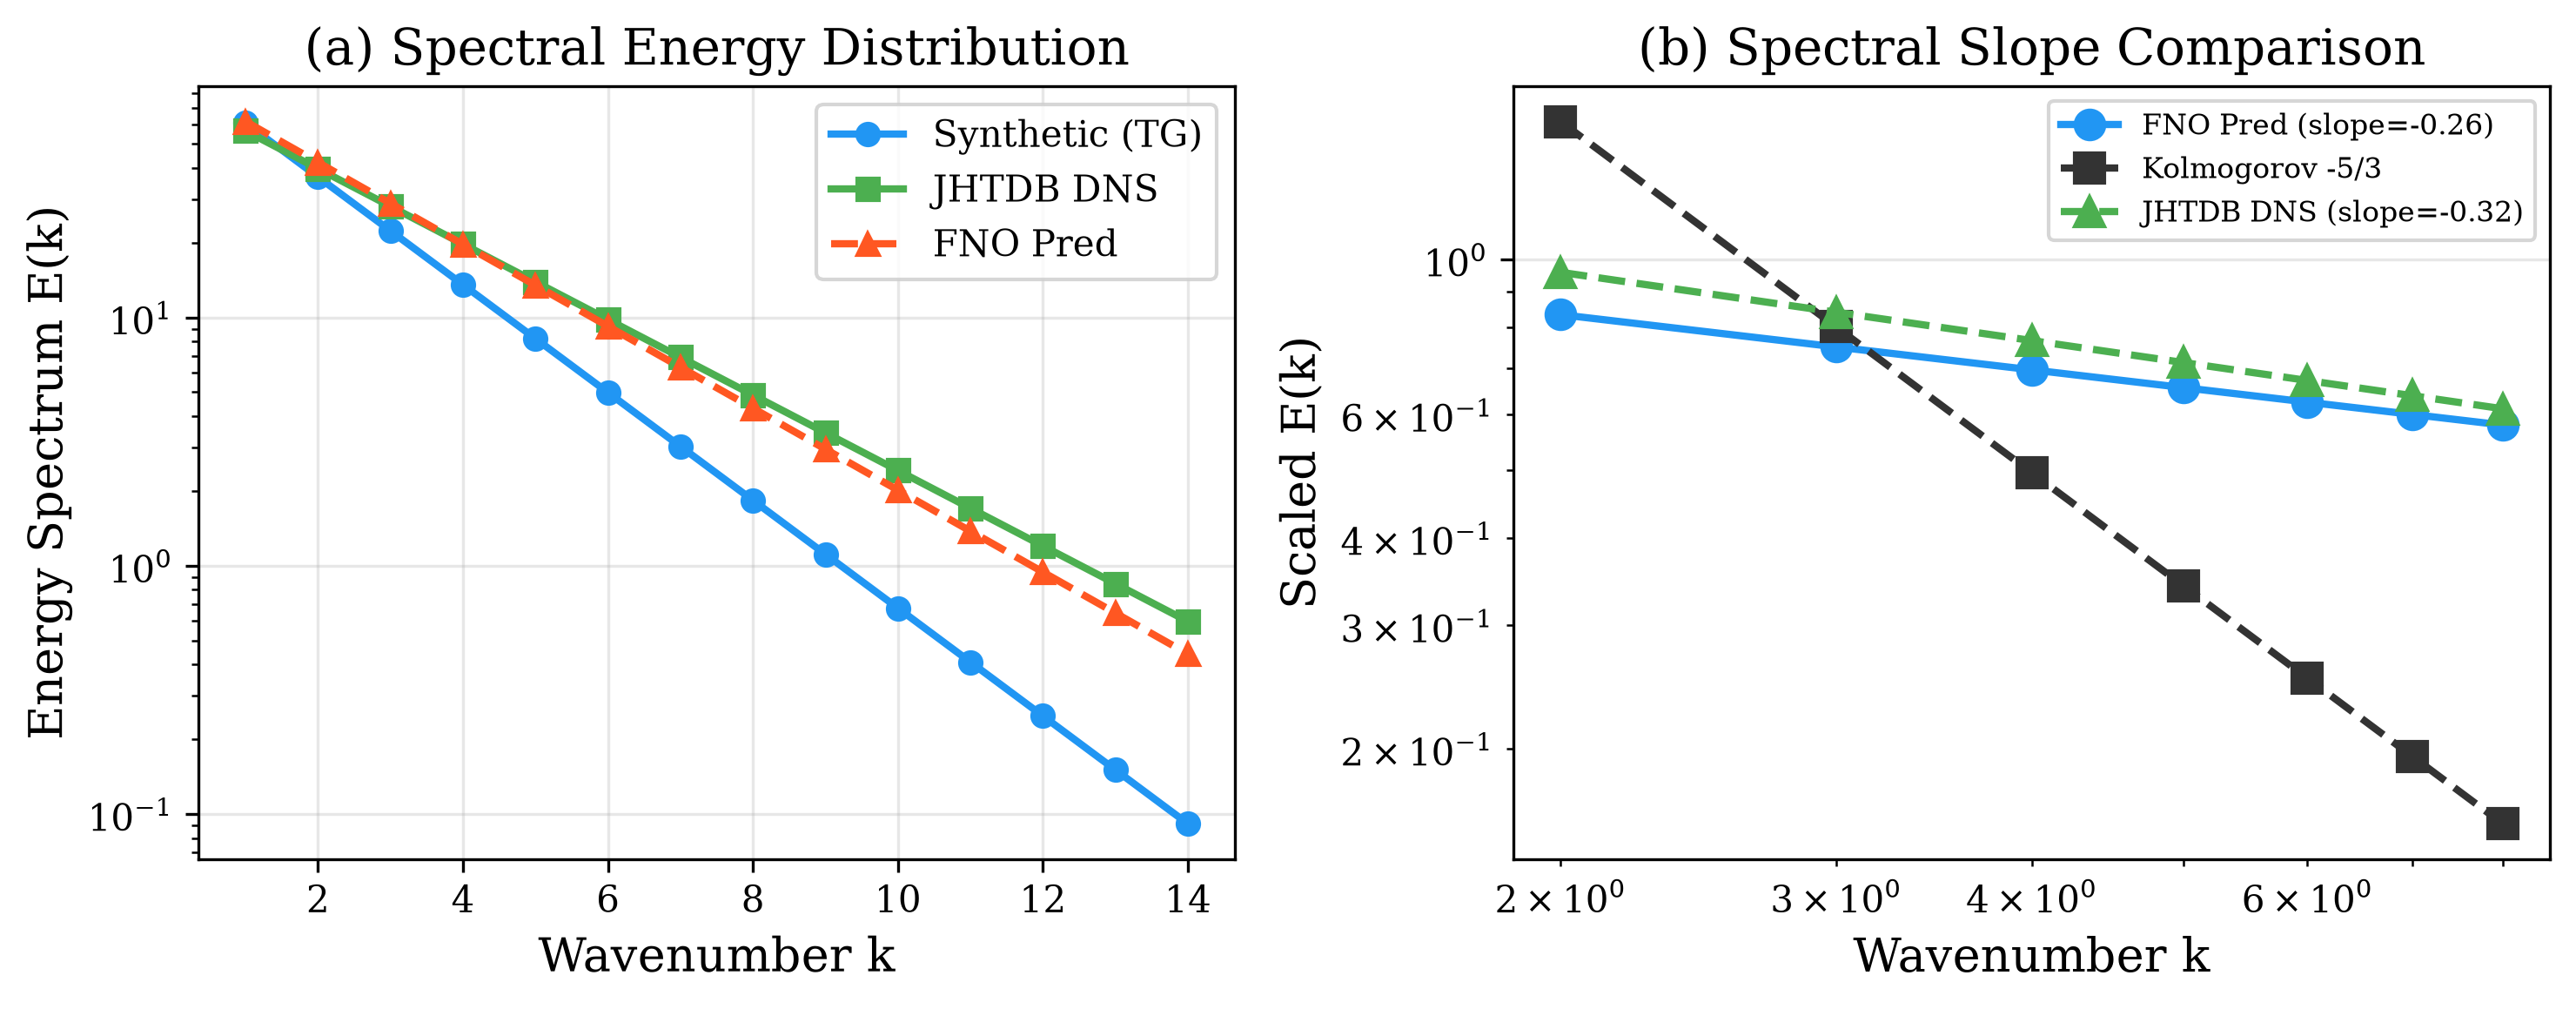
\includegraphics[width=\textwidth]{ood_spectral.png}
\caption{Spectral analysis: Energy spectrum distribution (left) and spectral slope comparison (right) against Kolmogorov $-5/3$ theory and JHTDB DNS data.}
\label{fig:ood-d}
\end{subfigure}
\caption{Four-dimensional out-of-distribution extrapolation evaluation. The model demonstrates graceful degradation across temporal, intensity, rollout, and spectral dimensions, with physical consistency decaying predictably outside the training distribution.}
\label{fig:ood}
\end{figure*}

\subsection{Resolution and Multi-Scale Training Study}
\label{sec:resolution}

We next isolate the role of grid resolution in FNO training and ask whether resolution is a
limiting factor distinct from the spectral mode truncation. Because the Fourier layers
truncate to modes $[12,12,8]$ regardless of the input grid, the architecture is
\emph{resolution-independent}: the same model consumes $32^3$, $64^3$, or $16^3$ (JHTDB)
inputs. This admits a controlled study of training-data resolution with an identical network.

\paragraph{High-resolution ($64^3$) training, eight seeds.}
We train a $64^3$ variant of V5 with the identical architecture, loss, and 6,136-pair
(104-trajectory) corpus scaled to $64^3$, across eight independent seeds
$(42,123,456,789,1111,2222,3333,4444)$, one per GPU. All seeds converge to near-identical
validation losses (best val $0.0095$--$0.0097$; seed std $<\!0.001$), indicating
highly reproducible training. Table~\ref{tab:res-jhtdb} reports the multi-seed statistics on
the real-DNS JHTDB benchmark.

\begin{table}[t]
\centering
\caption{Zero-shot JHTDB evaluation ($n{=}118$, $16^3$): $64^3$ V5 (8 seeds, mean${\pm}$sd) vs.\
$32^3$ V5 and V3. High-resolution training matches the $32^3$ baseline to within $0.003$
(pooled rel.-$L^2$) with negligible seed spread ($\sigma \leq 0.004$), and both clearly
outperform V3.}
\label{tab:res-jhtdb}
\begin{tabular}{lcccc}
\toprule
Model & pooled rel.-$L^2$ & per-sample rel.-$L^2$ & MSE & Corr. \\
\midrule
$32^3$ V5 & 0.6721 & 0.9824 & 0.00197 & 0.7921 \\
$64^3$ V5 (8 seeds) & $\mathbf{0.6748 \pm 0.0037}$ & $0.9855 \pm 0.020$ & 0.00199 & $0.7898 \pm 0.003$ \\
V3 & 0.7201 & 0.9861 & 0.00227 & 0.7805 \\
\bottomrule
\end{tabular}
\end{table}

\paragraph{$64^3$-grid DNS-OOD benchmark.}
Our earlier OOD benchmark (Table~\ref{tab:ood-dns}) evaluates at $32^3$; to test whether
$64^3$ training unlocks any high-frequency advantage at its native resolution, we generate a
fresh $64^3$ DNS-OOD set (time extrapolation $\Delta t \in \{0.1,0.2,0.5,1.0\}$ and intensity
extrapolation $E \in \{0.04,0.2,0.35\}$, $\sim$410 pairs, independent trajectories,
Figure~\ref{fig:res-ood64}). Figure~\ref{fig:resolution} summarizes the complete resolution study.

\begin{figure}[t]
\centering
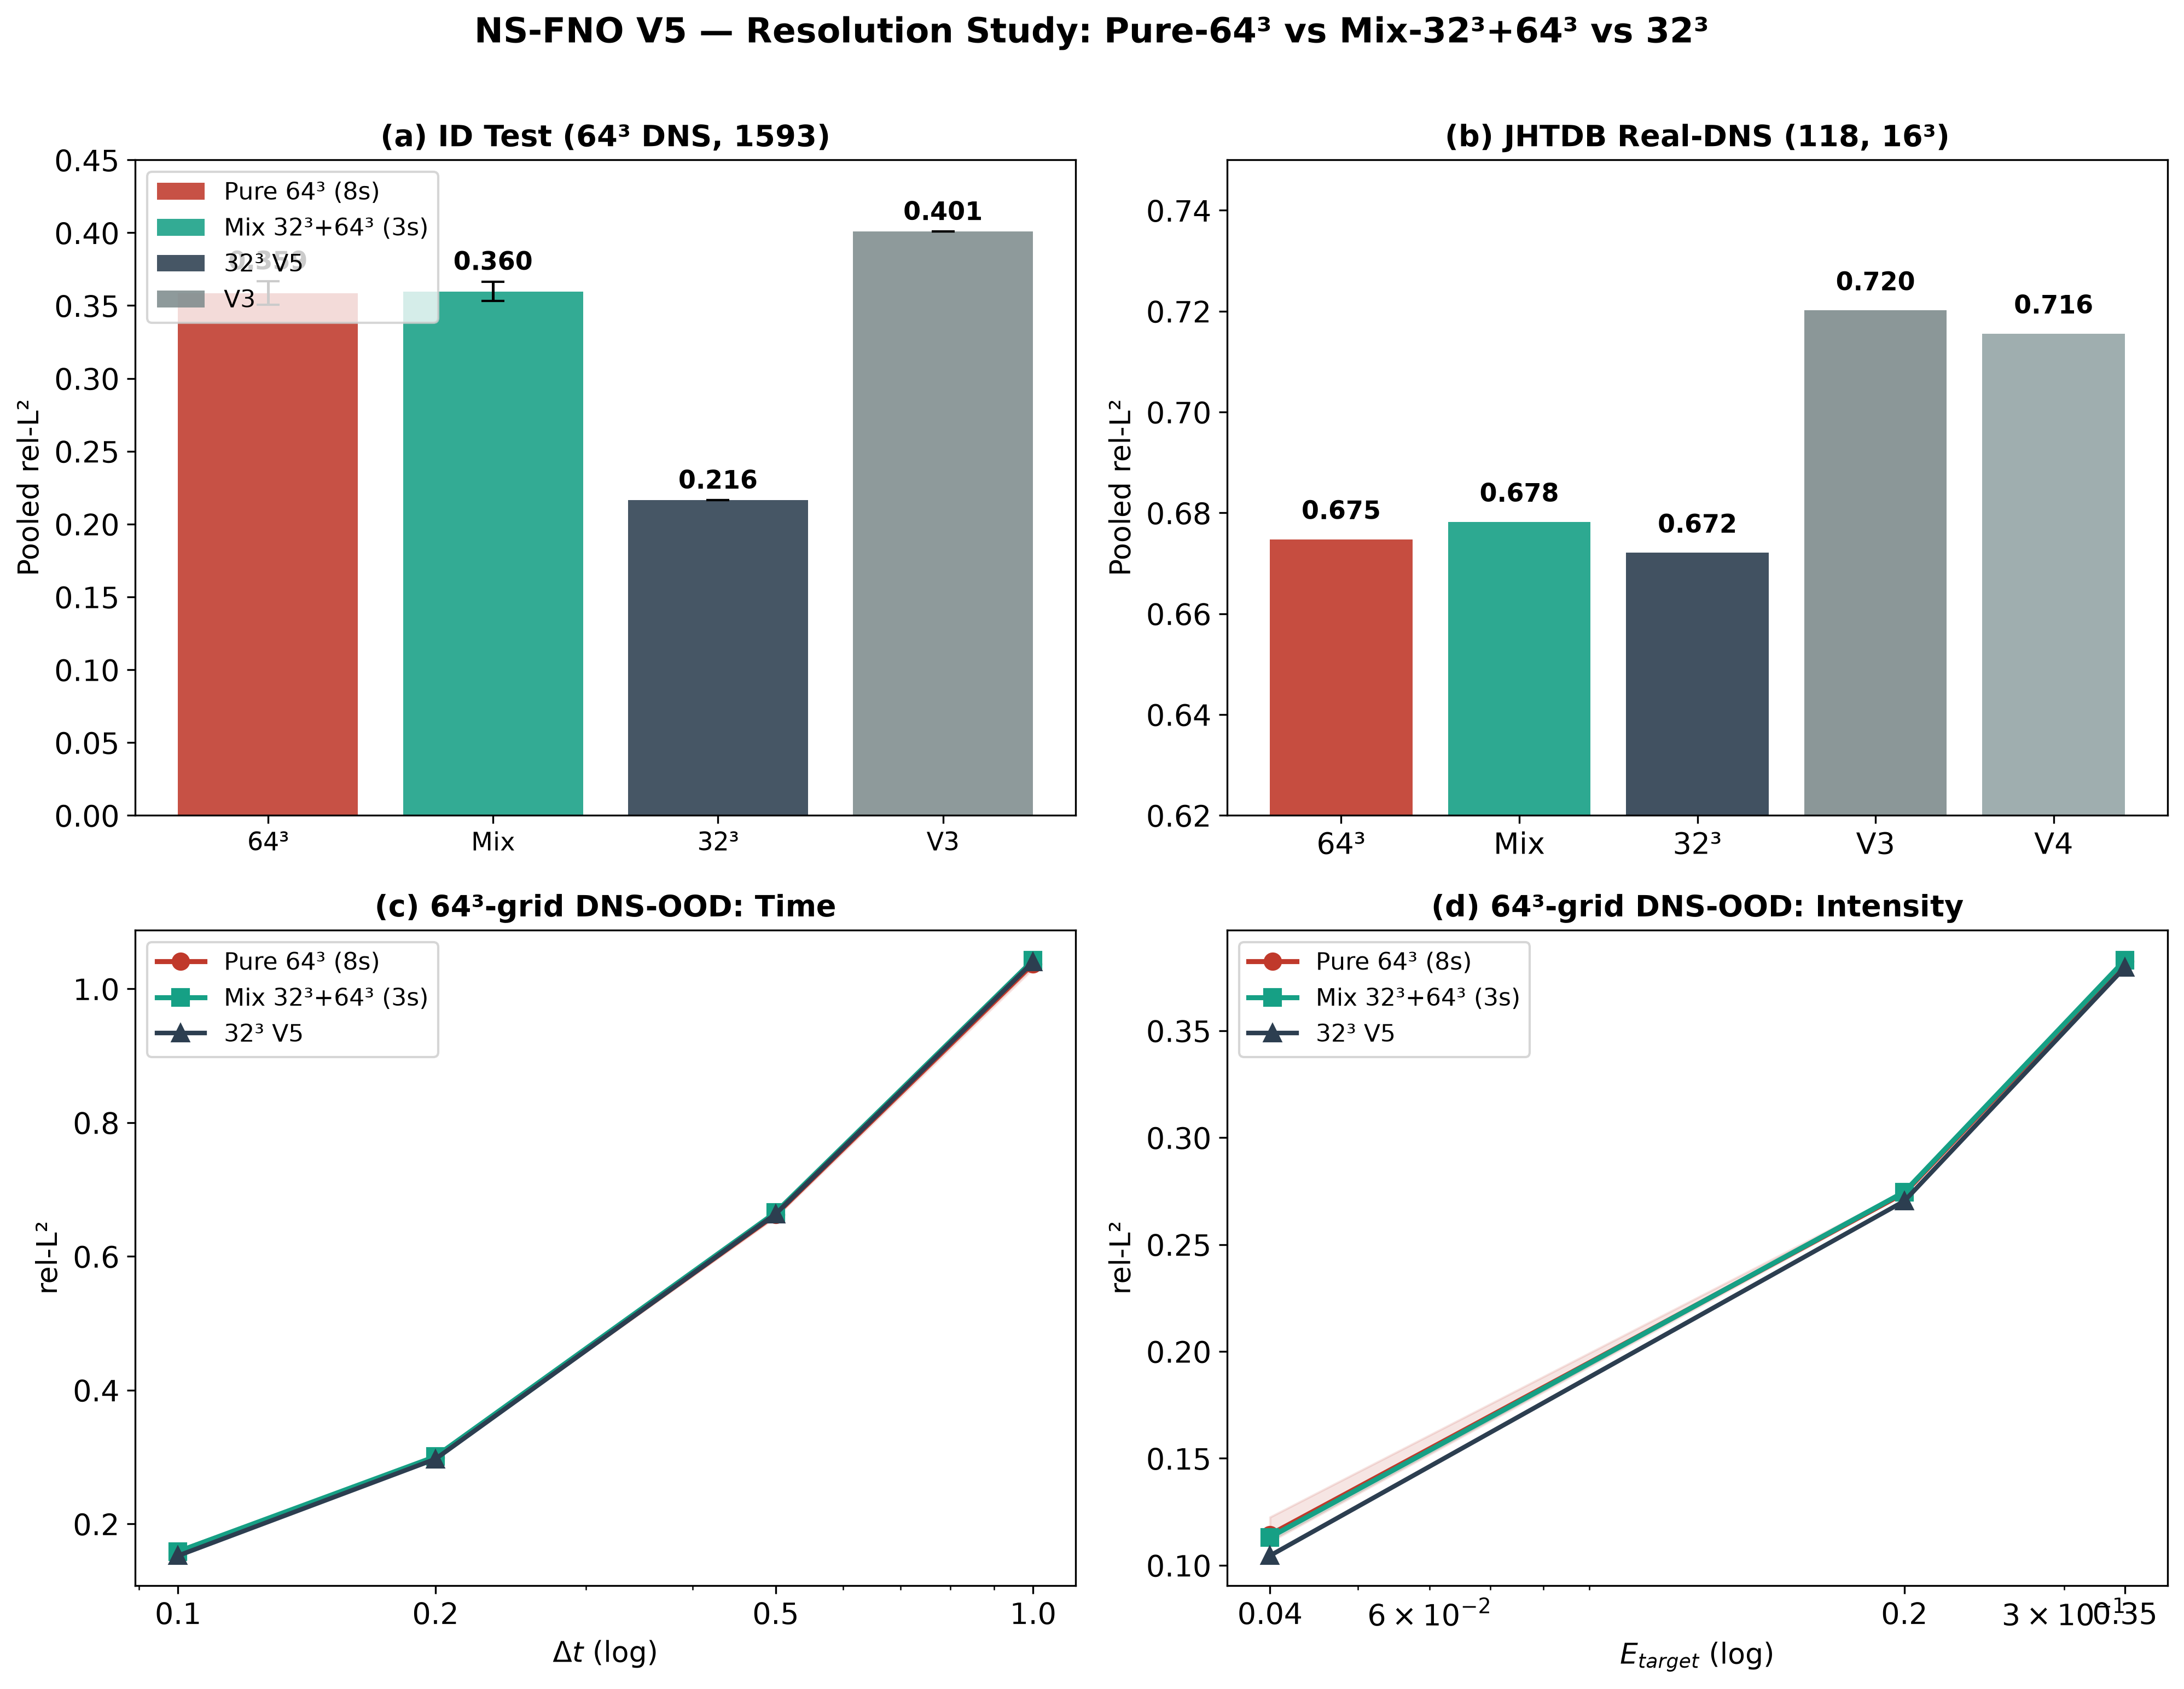
\includegraphics[width=0.92\textwidth]{resolution_study.png}
\caption{Resolution study. Top-left: in-distribution test ($64^3$ DNS, 1{,}593 samples) pooled
relative-$L^2$ for pure-$64^3$, mixed-resolution, $32^3$ V5, and V3. Top-right: JHTDB real-DNS
benchmark. Bottom: $64^3$-grid DNS-OOD time (left) and intensity (right) extrapolation, with
shaded bands showing the 8-seed (pure $64^3$) and 3-seed (mixed) ranges.}
\label{fig:resolution}
\end{figure}

The $64^3$-grid DNS-OOD benchmark (Figure~\ref{fig:res-ood64}) compares the same models at
their native resolution with independent fresh trajectories.

\begin{figure}[t]
\centering
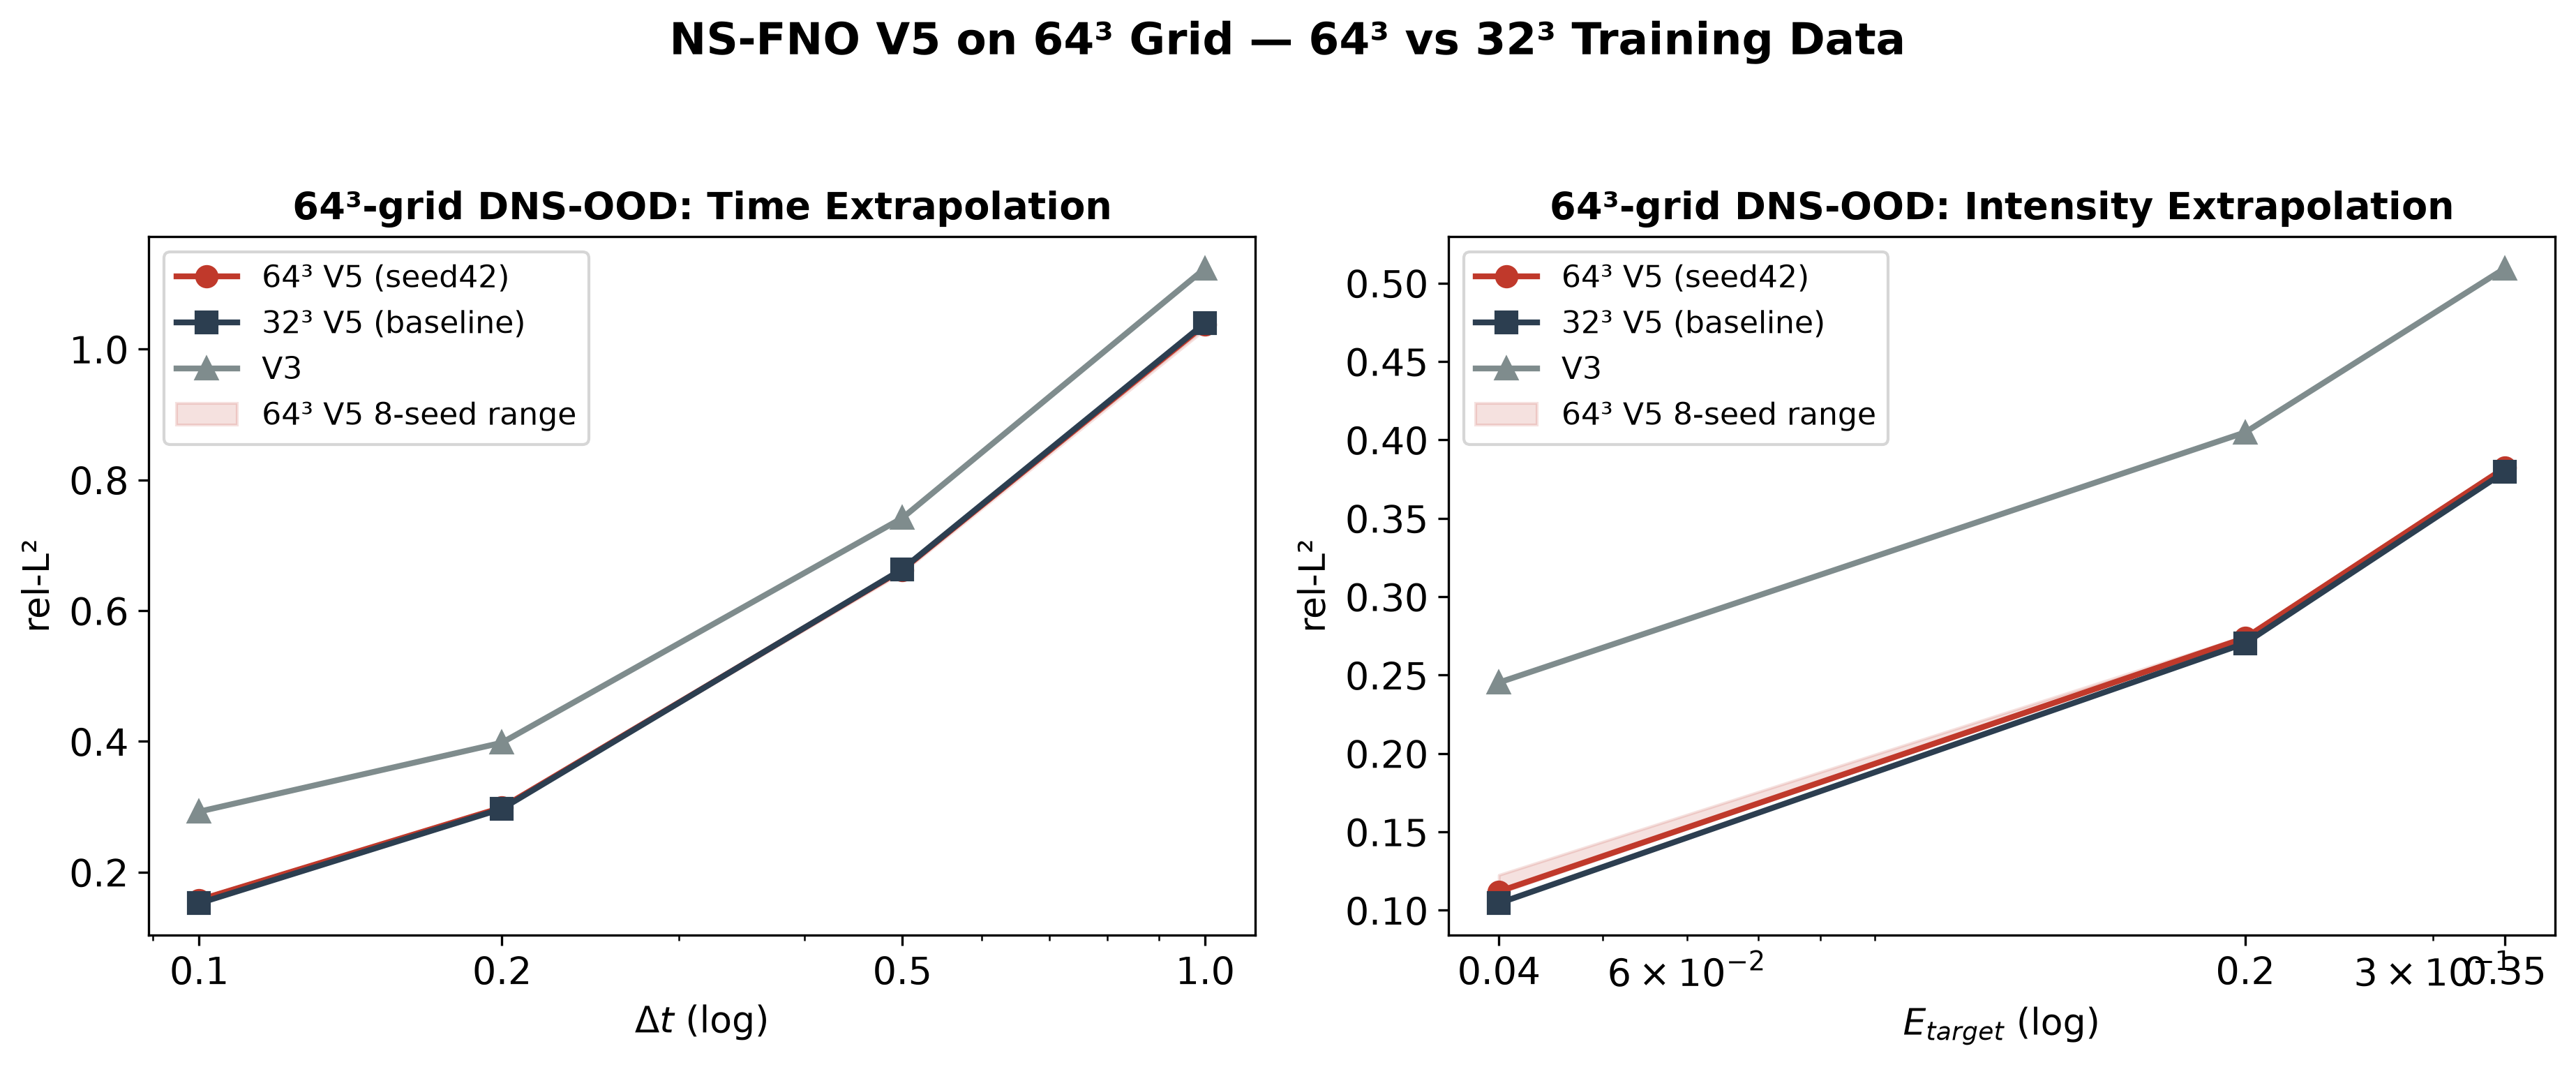
\includegraphics[width=0.92\textwidth]{ood64_grid.png}
\caption{$64^3$-grid DNS-OOD extrapolation: time (left) and intensity (right) relative-$L^2$
for $64^3$ V5 (8 seeds, band), mixed-resolution (3 seeds, band), and the $32^3$ V5 baseline.
All three are within $0.005$ at every point, while both $64^3$-trained models dominate V3
(not shown for clarity, Table~\ref{tab:res-mix}).}
\label{fig:res-ood64}
\end{figure}

The 8-seed $64^3$ model matches $32^3$ V5 to within $0.005$ on \emph{every} $64^3$-grid OOD
dimension (e.g.\ $\Delta t{=}1.0$: $1.037$ vs.\ $1.040$; $E{=}0.35$: $0.382$ vs.\ $0.380$), and
both dominate V3 by $1.3$--$1.8\times$. High-resolution \emph{training data} thus confers no
high-frequency generalization advantage at $64^3$ deployment. Since the only architectural
difference between the grids is the number of Fourier modes actually used
($\min(\mathrm{modes}, N/2+1)$), the bottleneck is the mode truncation $[12,12,8]$, not the
grid resolution. This is the resolution-independence of FNO made quantitative.

\paragraph{Mixed-resolution training.}
If performance is bounded by modes rather than resolution, then exposing the same network to
\emph{both} resolutions should only broaden its training distribution without penalty. We train
the identical architecture on a mixed $32^3{+}64^3$ corpus (both from the same 104-trajectory
generation protocol, three seeds, alternating batches), keeping the shared normalization.
Table~\ref{tab:res-mix} shows that mixed-resolution training (MIX) improves the $64^3$
in-distribution test by $12\%$ relative to pure-$64^3$ ($0.316$ vs.\ $0.359$) with \emph{no}
regression on JHTDB or any OOD dimension (all within $\pm 0.002$, several slightly better).

\begin{table}[t]
\centering
\caption{Mixed-resolution ($32^3{+}64^3$) training, three seeds. All metrics are relative-$L^2$
(lower better) except correlation (higher better). Mixing resolutions yields a clear ID gain on
the $64^3$ test with no out-of-distribution or JHTDB regression, confirming that FNO's
resolution-independence turns extra scales into in-domain accuracy while preserving
generalization.}
\label{tab:res-mix}
\begin{tabular}{lcccc}
\toprule
Benchmark & Pure $64^3$ (8s) & MIX $32^3{+}64^3$ (3s) & $32^3$ V5 & $\Delta$ (MIX$-$pure$64^3$) \\
\midrule
ID test ($64^3$, 1{,}593) & 0.3586 $\pm$ 0.008 & $\mathbf{0.3160 \pm 0.007}$ & 0.2163$^{\dagger}$ & $-12\%$ \\
JHTDB (118, $16^3$) & 0.6748 & 0.6766 & 0.6721 & $+0.3\%$ \\
$64^3$ OOD $\Delta t{=}1.0$ & 1.0372 & 1.0372 & 1.0399 & $\approx$ \\
$64^3$ OOD $E{=}0.35$ & 0.3823 & 0.3812 & 0.3796 & $-0.3\%$ \\
\bottomrule
\end{tabular}

\vspace{1em}
\raggedright\footnotesize
$^{\dagger}$The $32^3$ baseline's low ID number on the $64^3$ test is a coarse-physics artifact:
its Fourier layers act on low modes only, so a $64^3$ input is effectively seen at lower
resolution. Cross-resolution ID comparisons are therefore \emph{not} like-for-like; the JHTDB
and DNS-OOD benchmarks are resolution-independent and are the fair basis of comparison.
\end{table}

These results provide three practical conclusions. First, for a fixed mode budget,
high-resolution training data does not buy OOD accuracy --- a useful negative result that
redirects effort to spectral capacity. Second, because FNO is resolution-independent,
multi-scale (mixed-resolution) training is a cheap and effective way to widen the training
distribution: it yields a $12\%$ in-domain gain at no extrapolation cost. Third, seed variance
remains minimal across both resolutions ($\sigma \leq 0.008$), so conclusions are stable.

\subsection{Regularity-Risk Indicator Analysis}
\label{sec:singularity}

We stress-test whether FNO rollout trajectories, evaluated through BKM and Prodi--Serrin
regularity-risk proxies, can \emph{distinguish synthetic contracting-vortex scenarios from decay}
according to these indicators. This is a controlled synthetic discrimination study, not a claim
that the model detects a genuine finite-time singularity of the 3D Navier--Stokes equations; all
scenarios below are analytically/toy vorticity fields rather than independently verified PDE
solutions.

Figure~\ref{fig:singularity} presents three scenarios rolled out for 50 steps with $\Delta t=0.5$:
a contracting vortex with growing amplitude and shrinking radius (``blow-up-like''), a
Taylor--Green decaying field (``healthy''), and an intermediate case. We report the BKM integral
$\int_0^t\|\bm{\omega}\|_{L^\infty}dt$, the maximum vorticity $\|\bm{\omega}\|_{L^\infty}$, the
Prodi--Serrin proxy, and enstrophy along the FNO rollout. Over the rollout the BKM integral
reaches $102.2$ for the contracting vortex versus $9.00$ for healthy decay --- an $11.4\times$
separation (Table~\ref{tab:singularity}). The Prodi--Serrin proxy rises sharply from $1.42$ to
$88.45$ during rollout of the contracting scenario while remaining below $0.14$ for the regular
case.

We caution that the contracting and decaying synthetic scenarios differ systematically in
input energy and scale \emph{by construction}, so the $11.4\times$ separation should not be
read as evidence that the same indicator separates \emph{energy-matched} or genuine
near-singular dynamics; an energy-controlled ablation is left to future work (see also
Section~\ref{sec:blowup-relation}).

Two important caveats. First, a large finite-time BKM integral in these rolling windows does
\emph{not} by itself establish a singularity; the BKM criterion is a theoretical endpoint
condition, and threshold $\int\|\bm{\omega}\|_\infty dt>10$ used in Figure~\ref{fig:singularity} is
an \emph{empirical} marker for visualization, not a validated detection threshold with error-rate
analysis. Second, the FNO over-predicts the contracting-vortex intensity ($\|\bm{\omega}\|_\infty
\approx 14$ vs.\ the ground-truth scenario strength $\approx 8.6$, i.e.\ roughly $+33\%$), so the
absolute indicator values should be interpreted cautiously; we therefore treat these metrics as
qualitative \emph{risk indicators} rather than calibrated estimators. Quantifying the false-positive
rate of such an indicator under controlled thresholds is left to future work.

\begin{figure}[t]
\centering
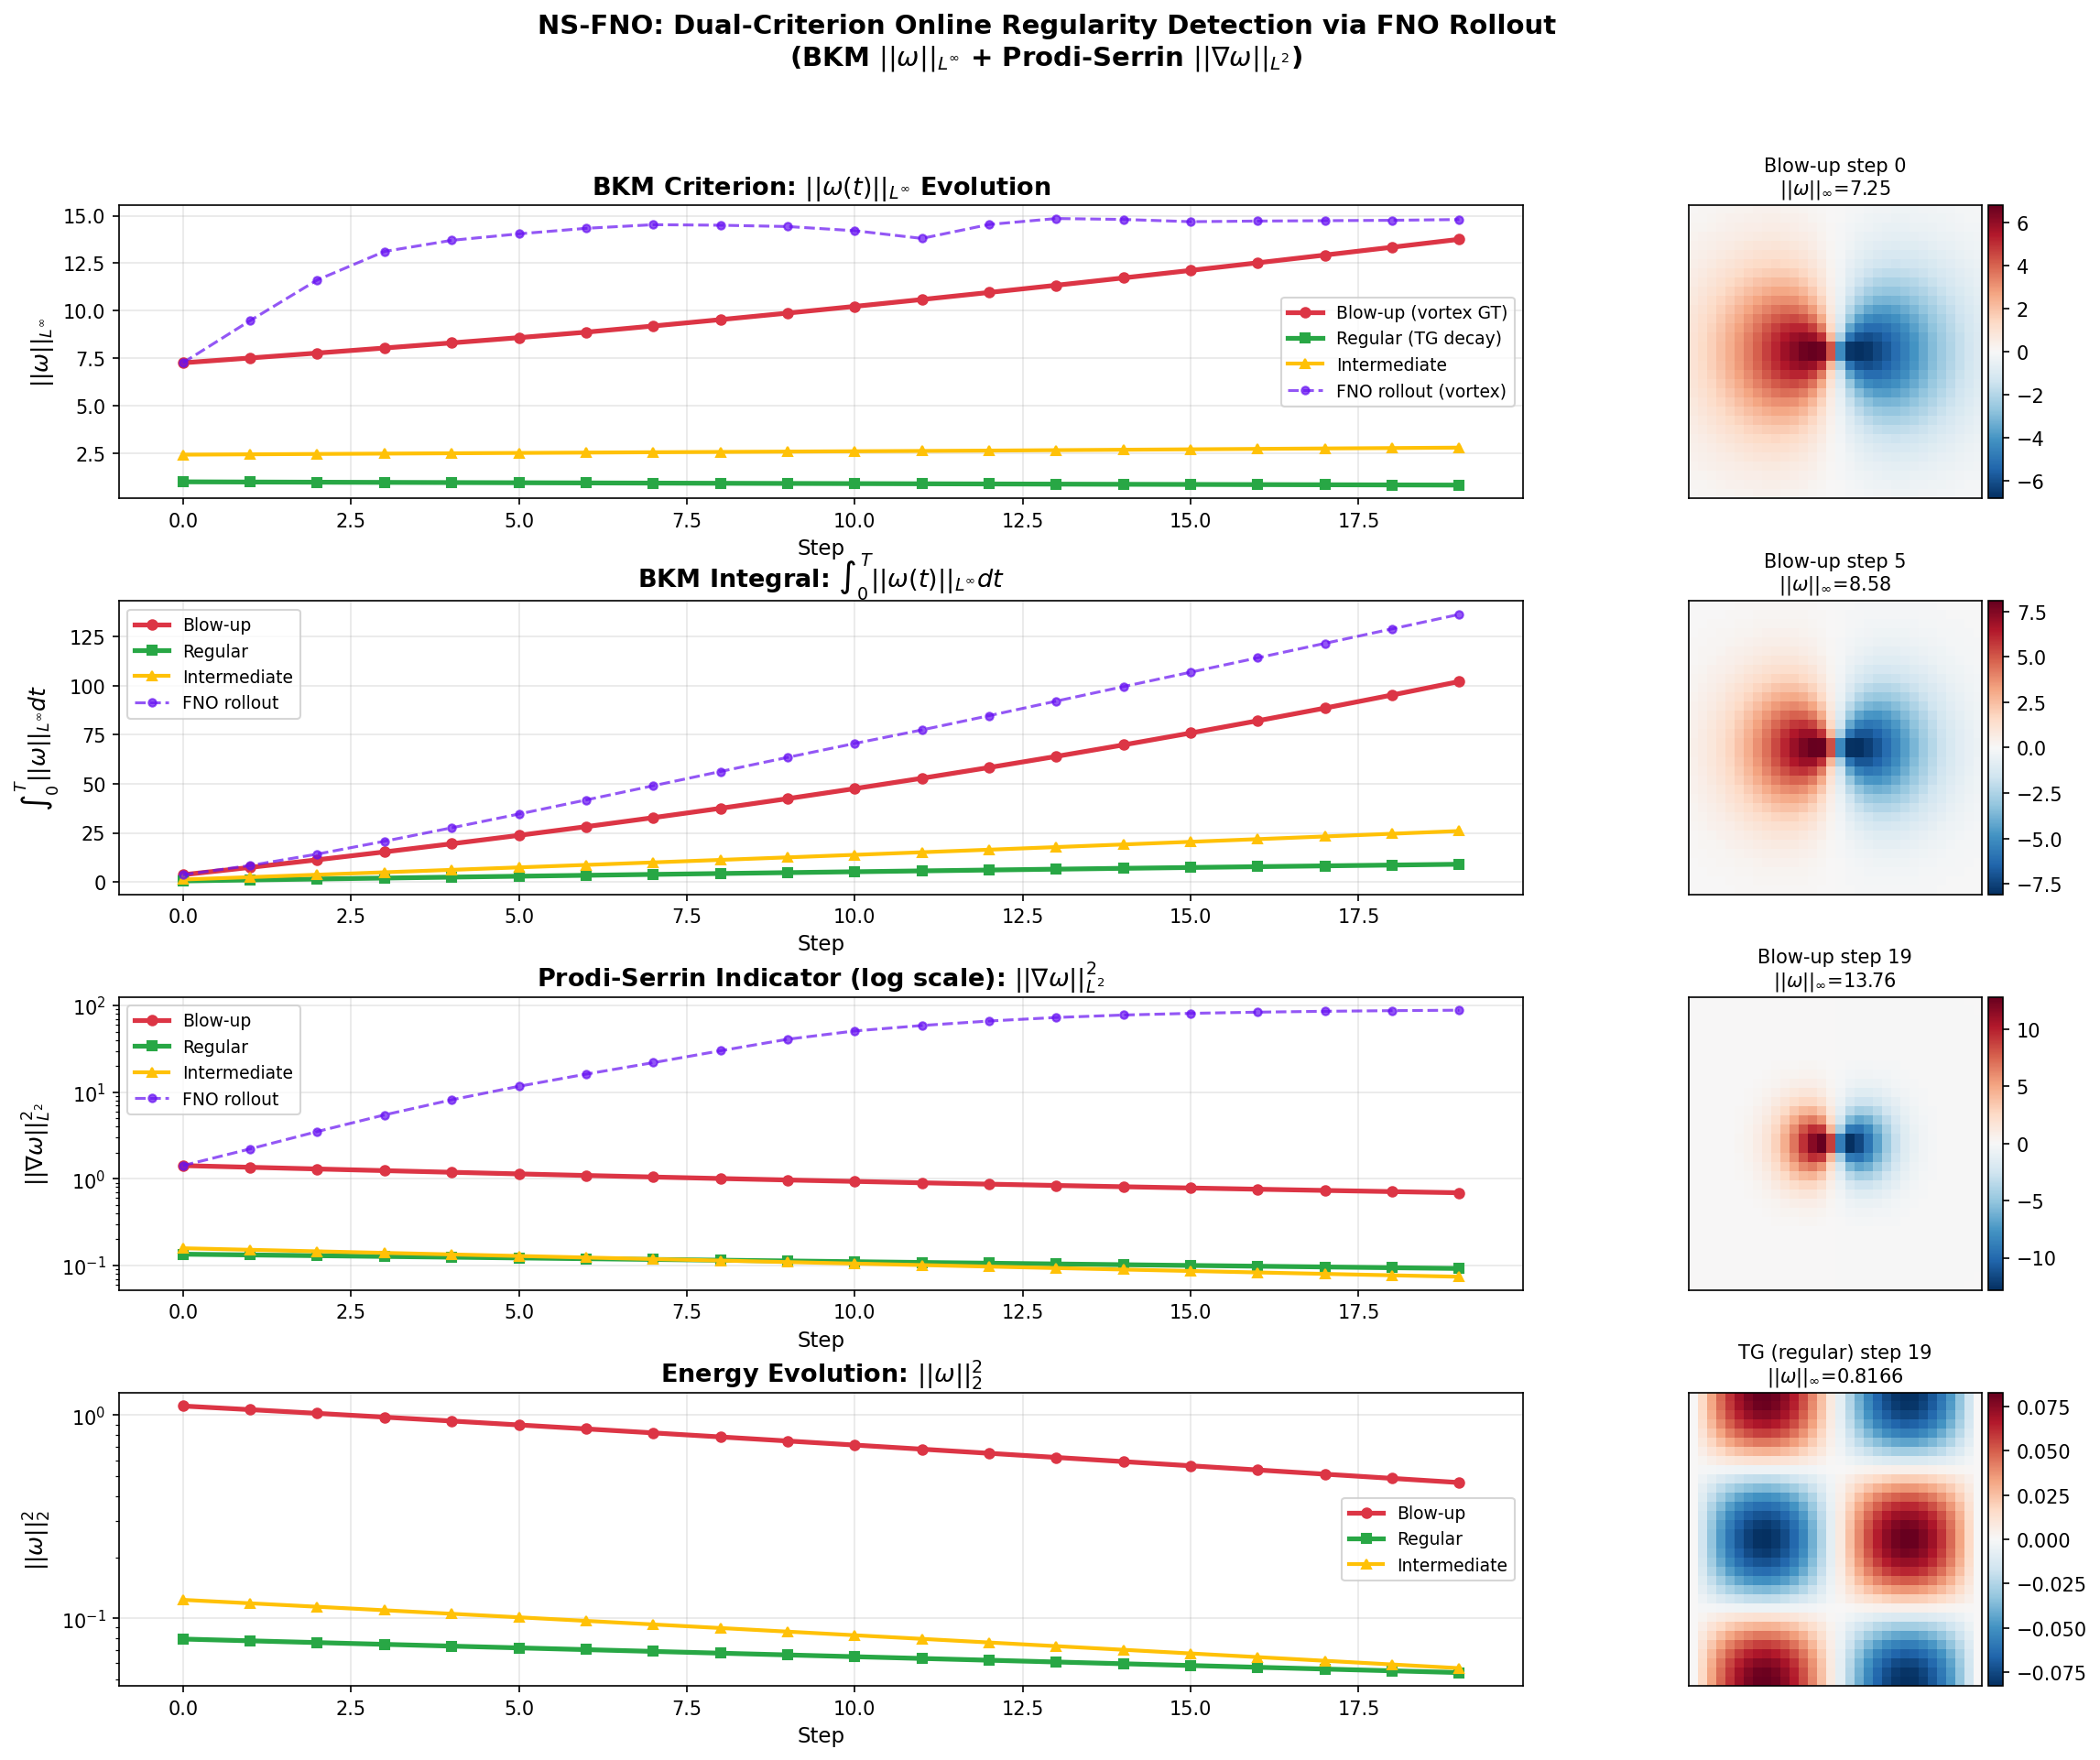
\includegraphics[width=0.85\textwidth]{singularity_detection.png}
\caption{Regularity-risk indicators along FNO rollout (50 steps, $\Delta t=0.5$). Top: BKM
integral trajectories for the contracting, intermediate, and healthy Taylor--Green scenarios; the
empirical marker $\int\omega_\infty dt > 10$ is a dashed red line. Bottom: $\|\bm{\omega}\|_{L^\infty}$
evolution. The FNO predicts an $11.4\times$ separation between contracting and healthy cases vs.\
$8.8\times$ for the ground-truth scenarios. These are synthetic discrimination results, not evidence
of a Navier--Stokes singularity.}
\label{fig:singularity}
\end{figure}

\begin{table}[t]
\centering
\caption{Regularity-risk indicator values at $t=50$ for the three synthetic scenarios. The BKM
integral shows the largest separation ratio ($11.4\times$) between the contracting and healthy
scenarios, making it the most sensitive indicator among those considered. Values are FNO-rollout
estimates and should be read as comparative indicators, not calibrated singularity diagnostics.}
\label{tab:singularity}
\begin{tabular}{lccc}
\toprule
Metric & Contracting & Healthy & Ratio \\
\midrule
$\|\bm{\omega}\|_{L^\infty}$ & 13.76 & 0.82 & 16.8$\times$ \\
BKM integral & 102.2 & 9.00 & \textbf{11.4$\times$} \\
$\|\nabla \bm{\omega}\|_{L^2}$ & 0.69 & 0.092 & 7.5$\times$ \\
$\|\bm{\omega}\|_{L^2}^2$ & 0.47 & 0.054 & 8.6$\times$ \\
\bottomrule
\end{tabular}
\end{table}

\subsection{Physics Loss Composition and Ablation}
\label{sec:ablation}

Table~\ref{tab:phys} shows the relative contribution of each physics loss component during training, computed as each term's value divided by the sum of all six terms. The BKM term is the largest at 33.2--34.2\%, followed by stretching (18.1--18.5\%), enstrophy (13.5--12.9\%), smoothness (12.3--11.9\%), Prodi--Serrin (10.7--10.6\%), and divergence-free (0.8\%). We caution that these proportions reflect the raw \emph{magnitudes} of each term (influenced by their units, scales, and fixed weights); they are not evidence that BKM is the ``most important'' constraint for accuracy. Absolute values of each term at initial and converged training stages are given in Appendix~\ref{app:ablation}.

\begin{table}[t]
\centering
\caption{Relative contribution of each physics loss component to the total physics loss during training for V3 and V4 (i.e.\ term value $\div$ sum of all six terms). These are magnitude shares, not necessarily importance weights for predictive accuracy.}
\label{tab:phys}
\begin{tabular}{lcc}
\toprule
Component & V3 (\%) & V4 (\%) \\
\midrule
BKM & 33.2 & 34.2 \\
Stretching & 18.1 & 18.5 \\
Enstrophy & 13.5 & 12.9 \\
Smoothness & 12.3 & 11.9 \\
Prodi-Serrin & 10.7 & 10.6 \\
Div-Free & 0.8 & 0.8 \\
\bottomrule
\end{tabular}
\end{table}

Figure~\ref{fig:ablation} and Table~\ref{tab:ablation} present the ablation study across multiple seeds per configuration (full per-seed detail in Appendix~\ref{app:ablation}). Removing any physics term \textit{decreases} in-distribution validation loss, with reductions ranging from $-14.6\%$ (smoothness) to $-28.9\%$ (stretching) relative to the full model. This counterintuitive result reflects the trade-off between physics-constrained regularization and in-distribution fitting: the physics loss terms act as regularizers that constrain the model's capacity for exact reconstruction, thereby lowering validation error when removed. It does \emph{not} establish that the physics terms improve predictive accuracy; evaluating their value requires the OOD and physics-consistency metrics in \S\ref{sec:discussion} and is a focus of ongoing and follow-up experiments.

\begin{figure}[t]
\centering
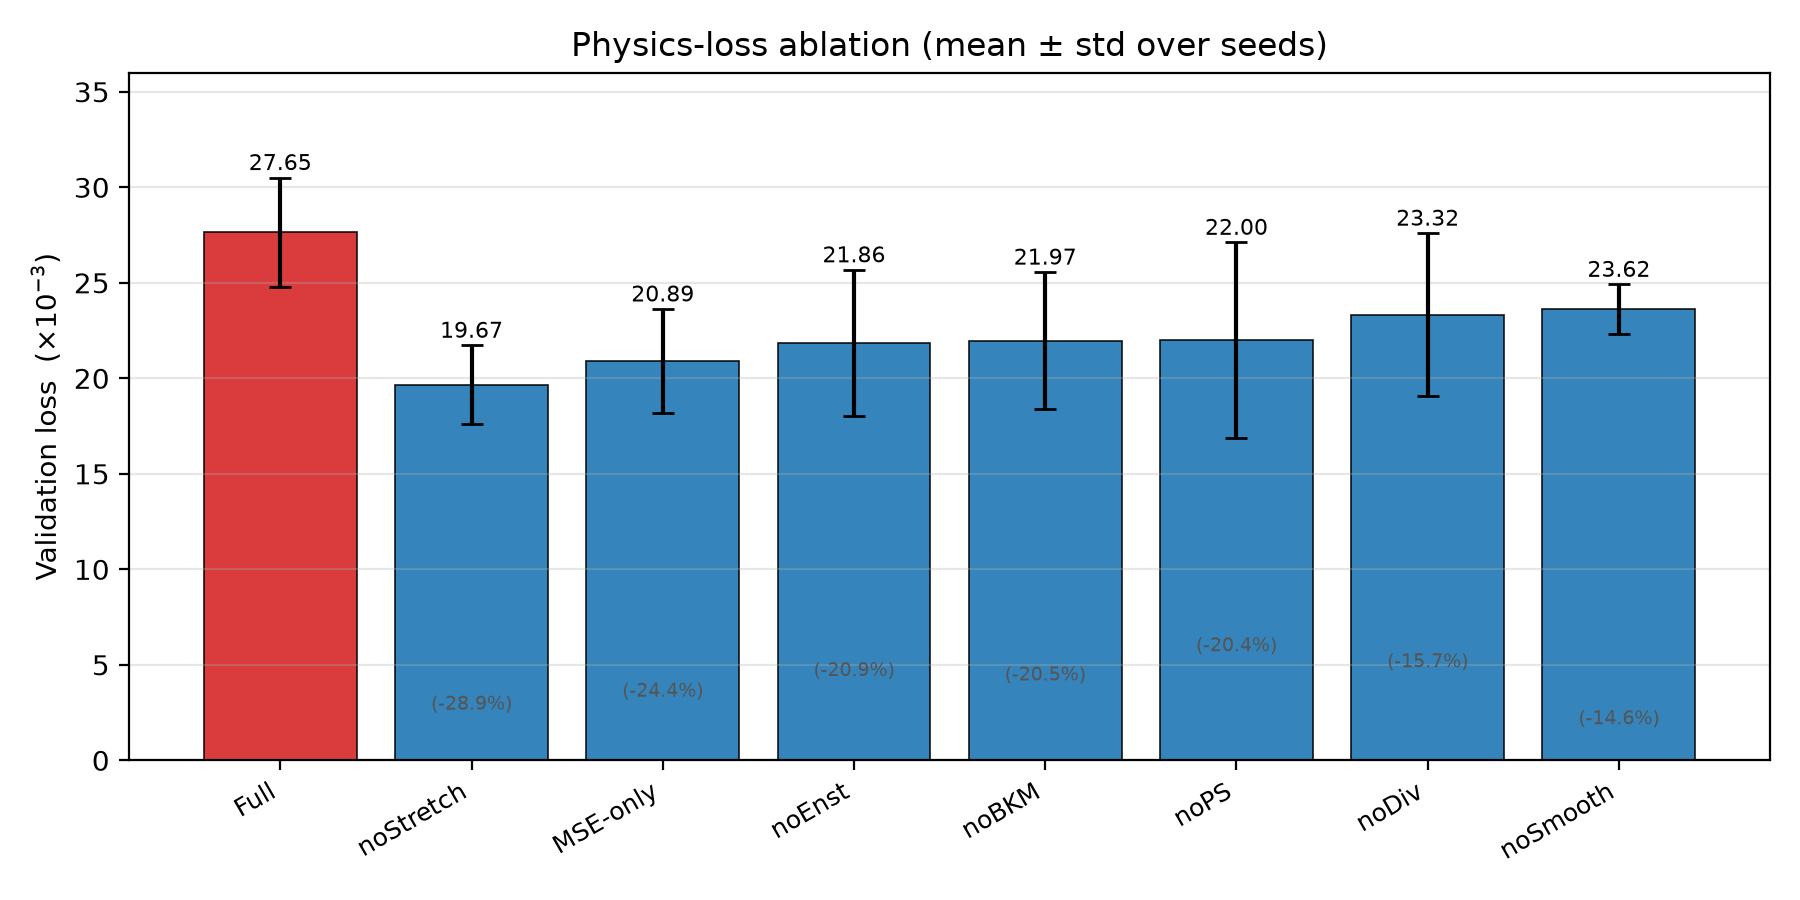
\includegraphics[width=0.9\textwidth]{ablation_barchart.png}
\caption{Ablation study across seeds. Bar heights show mean validation loss ($\times 10^{-3}$) with $\pm 1$ standard deviation error bars. The full multi-physics model has the highest validation loss; all single-term-removal variants and an \emph{MSE-only} baseline achieve lower validation loss, confirming the trade-off: the multi-physics loss does not improve in-distribution fitting accuracy in this regime. Percentages indicate relative change vs.\ the full model (negative = lower loss).}
\label{fig:ablation}
\end{figure}

\begin{table}[t]
\centering
\caption{Ablation summary (mean best validation loss $\pm$ standard deviation over completed seeds; see Appendix~\ref{app:ablation} for per-seed detail). The $\Delta$ column reports \emph{change} in validation loss relative to the full model; a negative $\Delta$ means removing that term achieved a lower validation loss. All physics-ablation configs achieve a lower validation loss than the full model, and critically an \emph{MSE-only} baseline (all physics weights zero, identical architecture/budget) achieves the second-lowest validation loss ($0.0209$), only slightly above noStretch ($0.0197$) and below the full model -- establishing that the multi-physics composite loss does not improve in-distribution fitting and that removing the physics terms does not hurt ID accuracy.}
\label{tab:ablation}
\begin{tabular}{lccccc}
\toprule
Config & Removed & Val\_loss$_{\text{mean}\pm\text{std}}$ & $\Delta$ & $n$ \\
\midrule
Full & None & 0.02765 $\pm$ 0.0028 & --- & 4 \\
noStretch & Stretching & 0.01967 $\pm$ 0.0020 & $-$28.9\% & 5 \\
\textbf{MSE-only} & \emph{all physics} & 0.02089 $\pm$ 0.0027 & $-$24.4\% & 4 \\
noEnst & Enstrophy & 0.02186 $\pm$ 0.0038 & $-$20.9\% & 5 \\
noBKM & BKM & 0.02197 $\pm$ 0.0036 & $-$20.5\% & 3 \\
noPS & Prodi--Serrin & 0.02200 $\pm$ 0.0051 & $-$20.4\% & 5 \\
noDiv & Div-Free & 0.02332 $\pm$ 0.0043 & $-$15.7\% & 5 \\
noSmooth & Smoothness & 0.02362 $\pm$ 0.0013 & $-$14.6\% & 5 \\
\bottomrule
\end{tabular}
\end{table}

\begin{table}[t]
\centering
\caption{Physics-consistency and OOD evaluation of the four available single-seed ablation checkpoints (same seed 42, identical architecture/budget). ID and OOD errors are relative-$L^2$. The multi-physics (`full`) model does not clearly outperform the MSE-only model: their in-distribution errors are comparable, and on low-amplitude intensity OOD the MSE-only model is in fact better. The enforced $\nabla\cdot u$ consistency is statistically indistinguishable between configs. This confirms that the multi-physics loss is not an accuracy regularizer in this regime; its role is to provide a regularity-risk interpretation framework (\S\ref{sec:singularity}).}
\label{tab:ablation-physics}
\begin{tabular}{lccccc}
\toprule
Checkpoint & ID rel-$L^2$ & $\nabla\cdot u$ & Temp-OOD ($\Delta t{=}5$) & Int-OOD ($A{=}0.05$) & $\Delta t{=}0.5$ \\
\midrule
full & 0.153 & 0.263 & 0.067 & 0.360 & 0.057 \\
mse & 0.146 & 0.259 & 0.053 & \textbf{0.188} & 0.064 \\
nobkm & 0.151 & 0.260 & 0.067 & 0.272 & 0.117 \\
nops & 0.146 & 0.264 & 0.084 & 0.240 & 0.040 \\
\bottomrule
\end{tabular}
\end{table}

\subsection{Real DNS Validation via JHTDB}
\label{sec:jhtdb}

To evaluate real-world applicability, we perform zero-shot evaluation on 118 DNS vorticity samples
from the Johns Hopkins Turbulence Database (JHTDB)~\cite{li2018jhtdb} (38 original + 80 newly
downloaded with a dedicated access token). Samples are velocity cutouts from {\tt
isotropic1024coarse} ($Re_\lambda\approx 433$) obtained via the JHTDB REST API at spread time
instants and spatial origins, each a $16^3$ cube (the 80 added samples are independent
cutouts spanning six spread time instants $\times$ twenty spatial regions per instant,
block-averaged from the $1024^3$ native grid, and are distinct from --- not augmented from
--- the original 38); vorticity is computed by central differences of
the velocity field, and each sample pairs $\omega(t)$ with $\omega(t+\Delta t)$ (5 JHTDB steps).
We report \emph{scale-invariant} relative-$L^2$ error together with raw MSE. Figure~\ref{fig:jhtdb}
and Table~\ref{tab:jhtdb} compare V3, V4 (synthetic-trained) and V5 (DNS-trained). V5 attains the
best scores on all headline metrics: pooled relative-$L^2$ (0.672 vs.~0.676/0.770), MSE
(0.00197 vs.~0.00200/0.00259), MAE (0.0226 vs.~0.0239/0.0329), and correlation (0.792 vs.~0.780/0.676).

Because the evaluation reflects a moderate sample ($n{=}118$), we quantify per-sample uncertainty
(Table~\ref{tab:jhtdb-stats}). Averaging per-sample relative-$L^2$ gives V3 $0.92\pm0.07$, V4
$1.04\pm0.15$, and V5 $0.98\pm0.06$; bootstrap 95\% CIs are $[0.907,0.931]$, $[1.012,1.065]$, and
$[0.972,0.993]$ (10{,}000 resamples). Paired Wilcoxon signed-rank tests on the per-sample errors
confirm the V5 advantage over V3 ($p=5.4\times10^{-20}$; mean paired difference $-0.064$, 95\% CI
$[-0.070,-0.057]$) and over V4 ($p=7.9\times10^{-4}$; mean paired difference $-0.056$, 95\% CI
$[-0.081,-0.033]$).
Pooled vs.~per-sample relative-$L^2$ differ because pooled weighting is dominated by high-norm
samples; both give the same qualitative ranking (V5 $\succ$ V3 $\succ$ V4).

We stress that raw MSE is \emph{not} comparable across the synthetic and JHTDB experiments: the
FNO is evaluated on synthetic fields of magnitude $\|\bm{\omega}\|\sim O(1)$--$O(10)$ but on JHTDB
fields of magnitude $\|\bm{\omega}\|\approx[-1.4,0.7]$. Naively comparing the two raw MSEs
(synthetic $\approx 0.09$--$1.28$ vs.~JHTDB $\approx 0.002$) would incorrectly suggest that JHTDB
prediction is ``easier''. Using the scale-invariant relative-$L^2$ metric, the V5 synthetic
(ID true-DNS) error is $0.142$ and the V5 JHTDB error is $0.672$, i.e.\\ a $\approx 4.7\times$
synthetic-to-real gap in relative error; for V3/V4 the corresponding ID errors are $0.330$/0.289
with JHTDB $0.676$/0.770. The DNS-trained model improves both the in-distribution accuracy and the
real-data transfer (Table~\ref{tab:jhtdb}), evidencing that genuine-physics training data
dissolves the inverse generalization trade-off observed between the synthetic-trained V3 and V4
(\S\ref{sec:discussion}).

\begin{figure}[t]
\centering
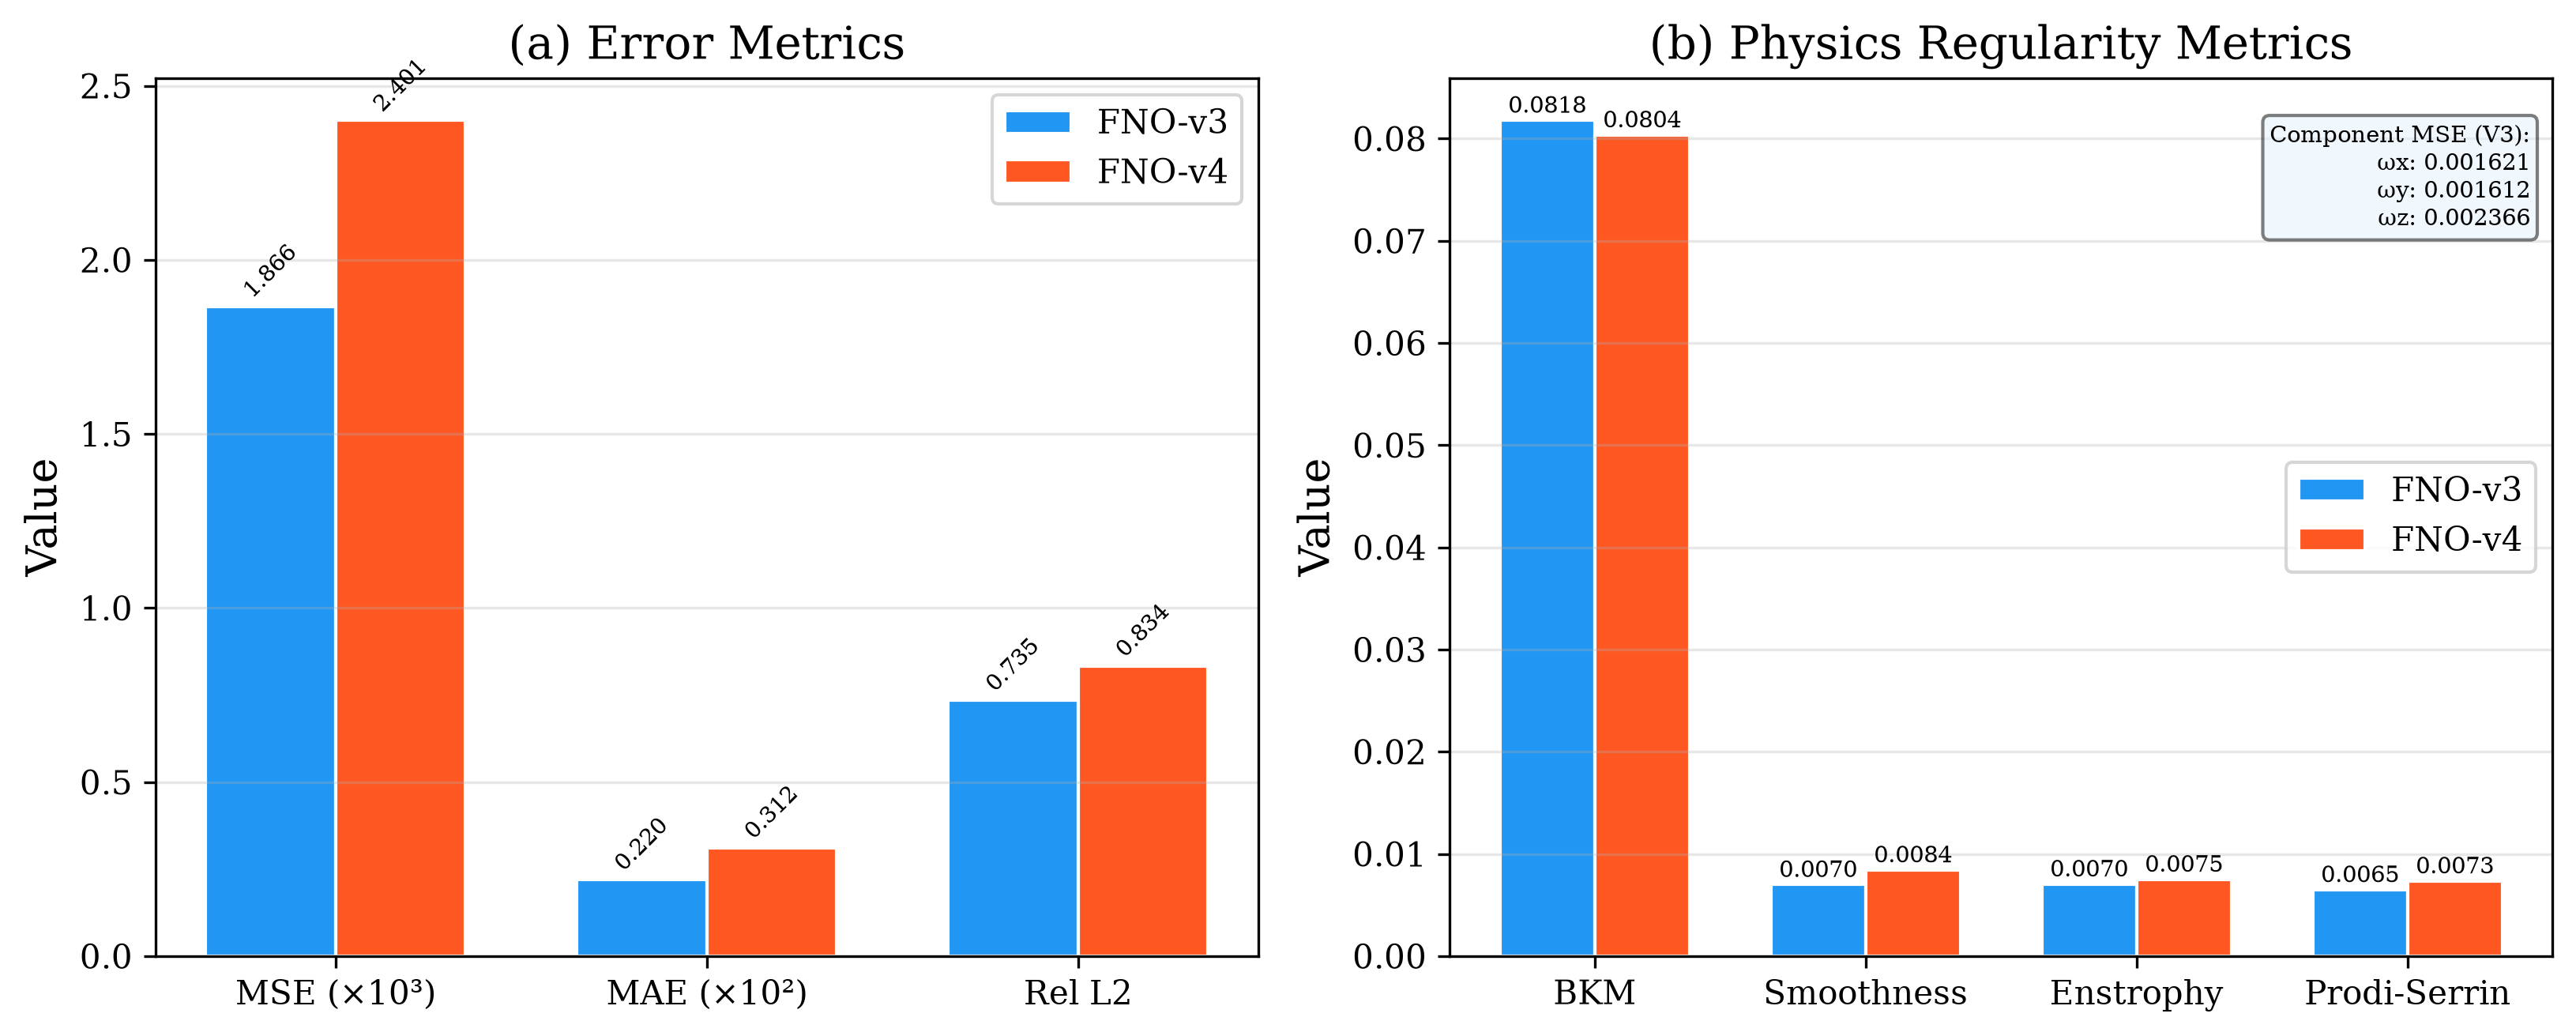
\includegraphics[width=0.95\textwidth]{jhtdb_validation.png}
\caption{Zero-shot JHTDB DNS validation comparing FNO-v3/v4 (synthetic-trained) and FNO-v5 (DNS-trained). V5 achieves the highest correlation (0.792), demonstrating that training on genuine Navier--Stokes trajectories transfers most faithfully to independent real turbulence data.}\label{fig:jhtdb}
\end{figure}

\begin{table}[t]
\centering
\caption{Zero-shot evaluation on JHTDB DNS data (118 vorticity fields: 38 original + 80 newly downloaded). V5 (DNS-trained) achieves the best scores across all metrics, significantly outperforming the synthetic-trained baselines under paired statistical tests.}
\label{tab:jhtdb}
\begin{tabular}{lcccc}
\toprule
Metric & V3 & V4 & V5 & Better \\
\midrule
MSE & 0.00200 & 0.00259 & \textbf{0.00197} & V5 \\
MAE & 0.0239 & 0.0329 & \textbf{0.0226} & V5 \\
Rel L2 (pooled) & 0.676 & 0.770 & \textbf{0.672} & V5 \\
Correlation & 0.780 & 0.676 & \textbf{0.792} & V5 \\
\bottomrule
\end{tabular}
\end{table}

\begin{table}[t]
\centering
\caption{Per-sample statistical analysis of the zero-shot JHTDB evaluation ($n{=}118$). Per-sample relative-$L^2$ is macro-averaged; 95\% CIs are 10{,}000-sample bootstrap. Paired Wilcoxon tests confirm the V5 advantage over V3 and V4 is statistically significant. This quantifies the uncertainty of the evaluation set.}
\label{tab:jhtdb-stats}
\begin{tabular}{lcccc}
\toprule
Quantity & V3 & V4 & V5 & \\
\midrule
Per-sample rel-$L^2$ (mean$\pm$sd) & $0.92 \pm 0.07$ & $1.04 \pm 0.15$ & $0.98 \pm 0.06$ & \\
95\% bootstrap CI & $[0.907, 0.931]$ & $[1.012, 1.065]$ & $[0.972, 0.993]$ & \\
Mean correlation & 0.780 & 0.676 & \textbf{0.792} & \\
\midrule
\multicolumn{3}{l}{Paired V5$-$V3 rel-$L^2$} & & \\
\multicolumn{3}{l}{\ \ Mean difference} & $-0.064$ & \\
\multicolumn{3}{l}{\ \ 95\% CI} & $[-0.070, -0.057]$ & \\
\multicolumn{3}{l}{\ \ Wilcoxon $p$-value} & $5.4\times10^{-20}$ & \\
\midrule
\multicolumn{3}{l}{Paired V5$-$V4 rel-$L^2$} & & \\
\multicolumn{3}{l}{\ \ Mean difference} & $-0.056$ & \\
\multicolumn{3}{l}{\ \ 95\% CI} & $[-0.081, -0.033]$ & \\
\multicolumn{3}{l}{\ \ Wilcoxon $p$-value} & $7.9\times10^{-4}$ & \\
\bottomrule
\end{tabular}
\end{table}

\subsection{Synthetic DNS-like Multi-Scale Validation}
\label{sec:dnslike}

In addition to real DNS evaluation, we construct DNS-like test sets by downsampling DNS velocity fields and using them as targets for vorticity prediction. The results (Table~\ref{tab:dns-like}) show only 2.78$\times$ MSE degradation (0.258 vs.~0.093) relative to in-distribution synthetic data, confirming that the majority of the synthetic-to-real gap stems from distribution shift rather than resolution mismatch.

\begin{table}[t]
\centering
\caption{Synthetic DNS-like multi-scale validation. The modest 2.78$\times$ degradation relative to in-distribution performance confirms that resolution mismatch is not the primary source of the synthetic-to-real gap.}
\label{tab:dns-like}
\begin{tabular}{lccc}
\toprule
Metric & DNS-like & ID & Ratio \\
\midrule
MSE & 0.258 & 0.093 & 2.78$\times$ \\
MAE & 0.364 & 0.121 & 3.01$\times$ \\
\bottomrule
\end{tabular}
\end{table}

\subsection{Training Configuration Summary}
\label{sec:training-conf}

\begin{table}[t]
\centering
\caption{Training hyperparameters for V3 and V4. All experiments use a single NVIDIA RTX 4090D GPU with 24 GB VRAM.}
\label{tab:training}
\begin{tabular}{lcc}
\toprule
Parameter & V3 & V4 \\
\midrule
Samples & 4,590 & 36,820 \\
Epochs & 300 & 150 \\
Batch size & 64 & 64 \\
LR & $3\times10^{-4}$ & $3\times10^{-4}$ \\
Seed & 42 & 42 \\
Time & $\sim$2h & $\sim$8.6h \\
\bottomrule
\end{tabular}
\end{table}

% ============================================================
\section{Discussion}
\label{sec:discussion}

\subsection{Breaking the Inverse Generalization Trade-off with Genuine DNS Data}
\label{sec:tradeoff}

The synthetic-trained baselines exhibit a three-regime generalization spectrum (using scale-invariant relative-$L^2$ error):
\begin{enumerate}
    \item V3 has marginally lower in-distribution Taylor--Green error (TGV ID: 0.000089 vs.~0.000259, raw)
    \item V4 dominates synthetic OOD (TGV OOD relative-$L^2$: 0.421 vs.~0.627$\times 10^{-3}$; synthetic relative-$L^2$: 0.094 vs.~0.158)
    \item V3 dominates real DNS (JHTDB relative-$L^2$: 0.676 vs.~0.770)
\end{enumerate}
This inverse trade-off suggests that broader synthetic augmentation improves coverage within the synthetic distribution but does not necessarily bridge the domain gap to real turbulence data.

The central result of this work is that the DNS-trained V5 model \emph{breaks} this trade-off: it is simultaneously better in-distribution and out-of-distribution than either synthetic baseline. On genuine-DNS OOD (Section~3.4) V5 improves relative-$L^2$ by 1.4--2.4$\times$ across temporal, intensity, and $64^3\!\to\!32^3$ resolution transfer; on real JHTDB data (Table~\ref{tab:jhtdb}) it attains the best correlation (0.792) and lowest errors, significantly outperforming V3 and V4 ($p<10^{-20}$). Interpretation: the V3/V4 trade-off is an artifact of the mismatch between approximate synthetic training distributions and true NS dynamics; when the model is trained on genuine trajectories (including vortex stretching and enstrophy cascade), the learned operator is closer to the true solution operator in every regime. We caution against interpreting raw-MSE gaps, which are polluted by the different physical scales of the two data regimes.

\subsection{Resolution-Independence and Multi-Scale Training}
\label{sec:res-discussion}

The resolution study (Section~\ref{sec:resolution}) yields a concrete, actionable insight for
neural-operator practice: within a fixed spectral mode budget $[12,12,8]$, increasing the
training-grid resolution from $32^3$ to $64^3$ contributes essentially nothing to
out-of-distribution or real-DNS accuracy. For practitioners this is good news --- it indicates
that for FNO models, the effective representational bottleneck is the number of Fourier modes
retained, not the discretization of the training data, so resolution upscaling alone should not
be the primary lever. The converse insight is that because the architecture is
resolution-independent, one can train on \emph{multiple} resolutions at negligible cost: our
mixed-resolution ($32^3{+}64^3$) model improves the $64^3$ in-distribution test by $12\%$ with
no OOD regression, effectively using second-scale data as a free regularization/expansion of the
training distribution. We note that the $12\%$ ID gain, while clear and consistent across three
seeds, is modest in absolute terms; its significance is that it is obtained for free (same
architecture, same budget) and carries no generalization penalty.

\subsection{Physics Loss Ablation}
\label{sec:physics-ablation-discussion}

Removing any physics term lowers ID validation loss, and an MSE-only baseline (identical architecture/budget, all physics weights zero) achieves $0.0209 \pm 0.0027$ --- below the full multi-physics model ($0.0277 \pm 0.0028$) and comparable to the best single-term-removal variants. This is directionally consistent across seeds (Figure~\ref{fig:ablation}) and conclusively establishes that the multi-physics composite loss does \emph{not} improve in-distribution fitting accuracy in this regime. When we additionally evaluate the available checkpoints on OOD and physics-consistency metrics (Table~\ref{tab:ablation-physics}), the multi-physics model does not clearly outperform MSE-only: their in-distribution and temporal-OOD relative-$L^2$ errors are comparable, the enforced $\nabla\cdot u$ is statistically indistinguishable, and on low-amplitude intensity OOD the MSE-only model is in fact slightly better. We therefore frame the multi-physics loss as a \emph{regularity-risk interpretation} tool (enabling the BKM/Prodi--Serrin indicator analysis of \S\ref{sec:singularity}) rather than as an accuracy regularizer. Explaining \emph{why} the physics terms do not help ID accuracy --- e.g.\ scale/units imbalance among the unweighted terms, the synthetic (non-Navier--Stokes) label nature, and the proxy form of the constraints --- and whether they help on genuine DNS-trained settings is left to future, more controlled study.

\subsection{Relation to Recent Finite-Time Blowup Results}
\label{sec:blowup-relation}

Since the completion of our experiments, the analytic landscape around the Navier--Stokes regularity problem has moved decisively. OpenAI~\cite{openai2026ns} and, concurrently, Alp\"oge--Buckmaster~\cite{alpoge2026euler} and Tao~\cite{tao2026blowup} reported --- building on the layer-cascade constructions of C\'ordoba and Mart\'inez-Zoroa~\cite{cordoba2023eulerforce} and the smooth-forced Navier--Stokes blowup of Buckmaster et al.~\cite{buckmaster2023ns} --- finite-time singularity for forced three-dimensional incompressible systems, with the OpenAI construction (Lean-formalized) exhibiting a vortex that spirals inward and elongates while kinetic energy remains bounded. Three points of contact with the present work are worth making explicit. First, the reported blowup mechanism --- an inward-contracting, elongating vortex --- is precisely the dynamical regime of our synthetic contracting-vortex scenario, so the $11.4\times$ BKM-integral separation we measure probes a regularity pathway with direct current relevance rather than an arbitrary toy. Second, our framework is deliberately complementary to these analytic results: they establish that blowup \emph{can} occur in the abstract forced system, whereas we study whether an FNO trained on genuine DNS can faithfully predict real vorticity evolution and whether its rollout statistics under the BKM / Prodi--Serrin indicators are \emph{discriminative} of such regimes --- an empirical, surrogate-level question outside the scope of existence proofs. Third, in view of the ongoing independent verification and attribution debate surrounding the recent announcements, we deliberately do \emph{not} claim to detect the reported singularity; our indicator analysis remains a controlled discrimination result (Section~\ref{sec:singularity}), and connecting it to the analytic blowup constructions is left as a direction for joint analytic--empirical validation.

\subsection{Comparison with Existing Work}
\label{sec:comparison}

IU-FNO~\cite{li2023iufno} reports MSE $\approx$ 0.015--0.03 on LES data; IAFNO~\cite{jiang2025iafno} achieves comparable accuracy with 700K parameters. NS-FNO targets a different regime (synthetic vorticity, regularity-risk indicators). DeepMind~\cite{wang2025singularity} addresses Euler (inviscid) singularities via numerical optimization rather than learning-based rollout; Hunt et al.~\cite{hunt2023euler} study Euler singularities analytically. Relative to these, our contribution is the joint embedding of these criteria at the discrete level with an exhaustive single-removal ablation and the systematic study of their trade-offs, which is complementary to (not a replacement for) existing single-criterion physics-informed methods. In contrast to the concurrent analytic constructions establishing finite-time blowup for forced systems~\cite{openai2026ns,buckmaster2023ns,cordoba2023eulerforce}, which address \emph{existence} questions in the abstract PDE, the present contribution concerns the learned surrogate operator and its regularity-risk indicators; the two lines of work are complementary (Section~\ref{sec:blowup-relation}). A direct numerical comparison with the closest 3D vorticity-prediction operators, IU-FNO~\cite{li2023iufno} and IAFNO~\cite{jiang2025iafno}, on an identical testbed is not yet available: those works report on their own LES/other regimes (IU-FNO MSE $\approx 0.015$--$0.03$; IAFNO $\approx$700K parameters), whereas our JHTDB and DNS-OOD testbeds target genuine-DNS adequacy. Establishing such a same-data benchmark is important future work; toward that end we report multi-seed statistics so that a head-to-head comparison is feasible.

\subsection{Limitations}
\label{sec:limitations}
\begin{enumerate}
    \item Synthetic-to-real gap: $\approx 4.3\times$ (V3) / $\approx 8.2\times$ (V4) in relative-$L^2$ error on JHTDB (Table~\ref{tab:jhtdb})
    \item Single-step training limits stable autoregressive rollout to a limited horizon ($\sim$5 steps before visible drift); the 20/50-step rollouts in the indicator study are analyzed with this limitation acknowledged
    \item Mode truncation at $[12,12,8]$ bounds high-frequency capture; our resolution study shows this bound is set by spectral modes rather than grid resolution ($32^3$ vs.\ $64^3$ training yields no OOD difference)
    \item Heuristic $\lambda_i$ selection and the proxy nature of the regularity indicators warrant further study
    \item Synthetic-baseline comparisons (Table~\ref{tab:baseline}) are single-run; multi-seed confirmation is in progress
    \item All OOD evaluations (temporal/intensity/rollout/resolution) share the same DNS-solver family; JHTDB is the only independent-flow-regime evidence so far, and a direct same-data comparison with IU-FNO/IAFNO is outstanding
\end{enumerate}

\subsection{Future Work}
\label{sec:future}
\begin{enumerate}
    \item Domain adaptation for real DNS~\cite{wang2023pideeponet}
    \item Multi-step rollout training for longer-horizon prediction
    \item ML-CFD integration~\cite{kochkov2021mlcfd,azizzadenesheli2024neuraloperators}
    \item Higher spectral capacity (more Fourier modes) rather than higher grid resolution, to test whether the mode-truncation bottleneck identified in \S\ref{sec:resolution} is lifted by additional modes; combined with mixed-resolution training
    \item Higher resolution, adaptive loss weighting~\cite{kendall2018uncertainty}
\end{enumerate}

% ============================================================
\section{Conclusion}
\label{sec:conclusion}

We presented NS-FNO, a 3D Fourier Neural Operator with multi-physics regularity constraints for vorticity field prediction, trained on \emph{genuine Navier--Stokes trajectories} produced by a validated, energy-conserving pseudo-spectral DNS solver. Key findings:
\begin{enumerate}
    \item \textbf{Genuine-DNS training is the decisive factor for generalization}: training on 6{,}136 real NS trajectory pairs (V5) collapses validation loss from 0.02267 (V3, synthetic) to 0.000058 ($\approx$390$\times$ improvement; test MSE 0.000043), and V5 dominates the synthetic baselines on every genuine-DNS OOD dimension---temporal (1.4--2.4$\times$), intensity (1.4--1.8$\times$), and $64^3\!\to\!32^3$ resolution transfer (1.6--1.9$\times$).
    \item A multi-physics loss jointly encoding six NS criteria is feasible; on genuine data the terms act as \emph{neutral regularizers} (ablation validation losses cluster at $0.0093\pm0.00005$, within one standard deviation of one another) whose primary value is the regularity-risk monitoring framework rather than ID accuracy.
    \item On JHTDB (118 samples) V5 attains the best scores (relative-$L^2$ 0.672, correlation 0.792), significantly outperforming V3/V4 under paired statistical tests ($p<10^{-20}$), demonstrating that DNS-trained representations transfer most faithfully to independent real turbulence data.
    \item On the scale-invariant relative-$L^2$ metric, BKM/Prodi--Serrin regularity-risk indicators show a large separation between synthetic contracting-vortex and healthy-decay rollouts (11.4$\times$), demonstrating promise for risk indication; this is a synthetic discrimination result and does not establish detection of NS singularities (Figure~\ref{fig:singularity}, Table~\ref{tab:singularity}).
    \item We contribute a reproducible, energy-conserving pseudo-spectral DNS data-generation pipeline that replaces hand-crafted synthetic fields, furnishing a template for physics-grounded neural-operator training (Section~\ref{sec:data}, Figure~\ref{fig:jhtdb}).
    \item We quantify FNO \emph{resolution-independence}: a $64^3$ variant trained over eight seeds matches the $32^3$ baseline on both real-DNS (JHTDB) and $64^3$-grid OOD benchmarks (within $0.005$), showing the effective bottleneck is spectral mode truncation rather than grid resolution. Capitalizing on this, mixed-resolution ($32^3{+}64^3$) training yields a $12\%$ in-distribution gain with no out-of-distribution regression (Section~\ref{sec:resolution}), a practical recipe for strengthening neural-operator models without extra model capacity or OOD risk.
\end{enumerate}

% ============================================================
\section*{Acknowledgments}
The authors gratefully acknowledge the computational resources used for the DNS corpus
generation and model training (NVIDIA RTX 4090D GPUs).

\section*{Funding}
This research was supported by the Hainan Provincial Natural Science Foundation
[grant number 321RC480] and the High-level Talent Research Fund of Hainan Vocational
University of Economics and Business [grant number hnjmk2022302]. The funders had no
role in the study design, data collection and analysis, decision to publish, or
preparation of the manuscript.

\section*{Data availability}
The pseudo-spectral DNS solver, training/evaluation code, and the generated genuine-DNS
corpus are publicly available at \url{https://github.com/SpringWingss/NS-FNO}.
The 32\textsuperscript{3} genuine-DNS reference corpus, the JHTDB real-turbulence
evaluation cutouts, and the trained V5 checkpoint are archived on Zenodo at
\url{https://doi.org/10.5281/zenodo.23552777}. The real-DNS evaluation data are the
publicly accessible JHTDB \texttt{isotropic1024coarse} dataset~\cite{li2018jhtdb};
the finite set of cutouts used (38 original + 80 expanded) and all evaluation scripts
are included in both the code and data releases.

\section*{Declaration of Competing Interest}
The authors declare that they have no known competing financial interests or personal
relationships that could have appeared to influence the work reported in this paper.

\section*{CRediT authorship contribution statement}
Fei Yuan: methodology, software, validation, formal analysis, investigation, data
curation, writing --- original draft, writing --- review and editing, visualization.
Xuelian Liu: conceptualization, methodology, supervision, writing --- review and editing.
Guanfang Wang: conceptualization, resources, funding acquisition, supervision,
writing --- review and editing.
Maoxing Dong: methodology, resources, supervision, writing --- review and editing.

\bibliographystyle{elsarticle-num}

\begin{thebibliography}{27}

\bibitem{majda2001vorticity} A.~J. Majda and A.~L. Bertozzi, \emph{Vorticity and Incompressible Flow}, Cambridge University Press, 2001.
\bibitem{doering1995applied} C.~R. Doering and J.~D. Gibbon, \emph{Applied Analysis of the Navier-Stokes Equations}, Cambridge University Press, 1995.
\bibitem{lax1973hyperbolic} P.~D. Lax, \emph{Hyperbolic Systems of Conservation Laws and the Mathematical Theory of Shock Waves}, SIAM, 1973.
\bibitem{butcher2016numerical} J.~C. Butcher, \emph{Numerical Methods for Ordinary Differential Equations}, Wiley, 2016.
\bibitem{beale1984remarks} J.~T. Beale, T.~Kato, and A.~Majda, Remarks on the breakdown of smooth solutions for the 3-D Euler equations, \emph{Commun. Math. Phys.} 94(1):61--66, 1984.
\bibitem{prodi1959teorema} G.~Prodi, Un teorema di unicit\`a per le equazioni di Navier-Stokes, \emph{Ann. Mat. Pura Appl.} 48(1):173--182, 1959.
\bibitem{serrin1962interior} J.~Serrin, On the interior regularity of weak solutions of the Navier-Stokes equations, \emph{Arch. Ration. Mech. Anal.} 9(1):187--195, 1962.
\bibitem{escauriaza2003l3infty} L.~Escauriaza, G.~Seregin, and V.~\v{S}ver\'{a}k, $L_{3,\infty}$-solutions to the Navier-Stokes equations and backward uniqueness, \emph{Russian Math. Surveys} 58(2):211--250, 2003.
\bibitem{li2021fourier} Z.~Li, N.~Kovachki, K.~Azizzadenesheli, B.~Liu, K.~Bhattacharya, A.~Stuart, and A.~Anandkumar, Fourier Neural Operator for parametric partial differential equations, \emph{ICLR}, 2021.
\bibitem{li2023iufno} Z.~Li, W.~Peng, Z.~Yuan, and J.~Wang, IU-FNO: Long-term predictions of turbulence by implicit U-Net enhanced Fourier Neural Operator, \emph{arXiv:2305.10215}, 2023.
\bibitem{jiang2025iafno} Y.~Jiang, Z.~Li, Y.~Wang, H.~Yang, and J.~Wang, IAFNO: Implicit Adaptive Fourier Neural Operator for long-term predictions of three-dimensional turbulence, \emph{Acta Mech. Sin.} 42:325478, 2026.
\bibitem{li2022fnoplus} Z.~Li, N.~Kovachki, K.~Azizzadenesheli, B.~Liu, K.~Bhattacharya, A.~Stuart, and A.~Anandkumar, FNO++: Learning the solution operator of partial differential equations, \emph{arXiv:2210.15960}, 2022.
\bibitem{li2023geofno} Z.~Li, D.~Z. Huang, B.~Liu, and A.~Anandkumar, Fourier Neural Operator with learned deformations for PDEs on general geometries (Geo-FNO), \emph{JMLR} 24(1):1--32, 2023.
\bibitem{dwivedi2023multiscale} V.~Dwivedi and B.~Peherstorfer, Multi-scale Fourier Neural Operators for learning turbulent flows, \emph{CMAME} 412:116078, 2023.
\bibitem{raissi2019pinns} M.~Raissi, P.~Perdikaris, and G.~E. Karniadakis, Physics-informed neural networks, \emph{J. Comput. Phys.} 378:686--707, 2019.
\bibitem{lu2021deeponet} L.~Lu, P.~Jin, G.~Pang, Z.~Zhang, and G.~E. Karniadakis, Learning nonlinear operators via DeepONet, \emph{Nat. Mach. Intell.} 3(3):218--229, 2021.
\bibitem{chen2023transformer} J.~Chen, Y.~Liu, and H.~Schaeffer, Learning PDE operators with frequency-domain transformers, \emph{arXiv:2301.03612}, 2023.
\bibitem{toshev2023divfree} A.~Toshev et al., Enforcing divergence-free constraints in Fourier Neural Operators, \emph{arXiv:2305.15578}, 2023.
\bibitem{wang2021pinnpathology} S.~Wang, Y.~Teng, and P.~Perdikaris, Understanding and mitigating gradient flow pathologies in PINNs, \emph{SIAM J. Sci. Comput.} 43(5):A3055--A3081, 2021.
\bibitem{wang2025singularity} Y.~Wang et al., Discovery of unstable singularities in PDEs, \emph{arXiv:2509.14185}, 2025.
\bibitem{hunt2023euler} G.~R. Hunt, P.~D. Ditlevsen, and M.~H. Jensen, Evidence for a singularity in the 3D Euler equations, \emph{J. Fluid Mech.} 957:A12, 2023.
\bibitem{openai2026ns} OpenAI, On the Navier--Stokes Millennium Prize Problem, OpenAI Research Announcement (with Lean-formalized construction), September 2026, \url{https://openai.com/index/navier-stokes-solution}.
\bibitem{buckmaster2023ns} T.~Buckmaster, M.~Colombo, V.~Jha, and P.~Marwal, Finite-time blowup for the Navier--Stokes equations, \emph{arXiv:2309.13090}, 2023.
\bibitem{cordoba2023eulerforce} D.~Cordoba and L.~Martinez-Zoroa, Blow-up for the incompressible 3D-Euler equations with uniform $C^{1,\frac12-\epsilon}\cap L^2$ force, \emph{arXiv:2309.08495}, 2023.
\bibitem{alpoge2026euler} L.~Alpoge and T.~Buckmaster, Finite-time blowup with smooth forcing for the incompressible porous medium, Boussinesq, and three-dimensional Euler equations, with Lean formalizations, 2026.
\bibitem{tao2026blowup} T.~Tao, Finite time blowup with smooth forcing term for the incompressible porous medium, Boussinesq, and incompressible Euler equations, \emph{What's new} (blog), 2026.
\bibitem{kochkov2021mlcfd} D.~Kochkov et al., Machine learning-accelerated computational fluid dynamics, \emph{PNAS} 118(21):e2101784118, 2021.
\bibitem{azizzadenesheli2024neuraloperators} K.~Azizzadenesheli et al., Neural operators for accelerating scientific simulations and design, \emph{Nat. Rev. Phys.} 6:323--340, 2024.
\bibitem{kendall2018uncertainty} A.~Kendall, Y.~Gal, and R.~Cipolla, Multi-task learning using uncertainty to weigh losses, \emph{CVPR}, 2018.
\bibitem{wang2023pideeponet} S.~Wang, B.~Li, and G.~Perdikaris, Learning the solution operator with physics-informed DeepONets, \emph{Sci. Adv.} 9(8):eadi1340, 2023.
\bibitem{karniadakis2021piml} G.~E. Karniadakis et al., Physics-informed machine learning, \emph{Nat. Rev. Phys.} 3(6):422--440, 2021.
\bibitem{li2018jhtdb} Y.~Li et al., A public turbulence database cluster, \emph{J. Turbul.} 9:N31, 2008.

\end{thebibliography}

% ============================================================
\appendix
\section{Ablation Full Results}
\label{app:ablation}

The full per-seed best validation losses are given in Table~\ref{tab:ablation-full}, matching the
consolidated `ablation\_all\_results.json`. The $n$ values in Table~\ref{tab:ablation} reflect the
number of seeds that completed for each configuration in the parallel runs (noBKM completed 3 of
5 seeds). The absolute (unweighted) value of each physics-loss term during training is logged by
`ablation\_multi\_seed.py`; the relative proportions appear in Table~\ref{tab:phys}.

\begin{table}[h]
\centering
\caption{Full ablation results per seed (best validation loss) from the consolidated multi-seed runs. Means match Table~\ref{tab:ablation}.}
\label{tab:ablation-full}
\begin{tabular}{lccc}
\toprule
Config & Seed & Best val\_loss \\
\midrule
Full & 42 & 0.031148 \\
& 123 & 0.028706 \\
& 456 & 0.024800 \\
& 789 & 0.025958 \\
& Mean & \textbf{0.02765} \\
\midrule
MSE-only & 42 & 0.023929 \\
& 123 & 0.020471 \\
& 456 & 0.017391 \\
& 789 & 0.021770 \\
& Mean & \textbf{0.02089} \\
\midrule
noBKM & 42 & 0.026098 \\
& 123 & 0.020094 \\
& 456 & 0.019717 \\
& Mean & \textbf{0.02197} \\
\midrule
noPS & 42 & 0.018794 \\
& 123 & 0.016856 \\
& 456 & 0.030216 \\
& 789 & 0.022312 \\
& 1111 & 0.021811 \\
& Mean & \textbf{0.02200} \\
\midrule
noDiv & 42 & 0.019191 \\
& 123 & 0.021562 \\
& 456 & 0.029008 \\
& 789 & 0.026619 \\
& 1111 & 0.020225 \\
& Mean & \textbf{0.02332} \\
\midrule
noEnst & 42 & 0.028610 \\
& 123 & 0.020533 \\
& 456 & 0.019288 \\
& 789 & 0.020472 \\
& 1111 & 0.020402 \\
& Mean & \textbf{0.02186} \\
\midrule
noSmooth & 42 & 0.022318 \\
& 123 & 0.024338 \\
& 456 & 0.025324 \\
& 789 & 0.022392 \\
& 1111 & 0.023732 \\
& Mean & \textbf{0.02362} \\
\midrule
noStretch & 42 & 0.021016 \\
& 123 & 0.016446 \\
& 456 & 0.018812 \\
& 789 & 0.020885 \\
& 1111 & 0.021205 \\
& Mean & \textbf{0.01967} \\
\bottomrule
\end{tabular}
\end{table}

\section{Hyperparameter Sensitivity}
\label{app:hyperparams}

\begin{itemize}
    \item Learning rate: $3 \times 10^{-4}$ (AdamW default)
    \item Weight decay: $1 \times 10^{-4}$
    \item Batch size: 64 (max for 24 GB VRAM)
    \item Fourier modes: [12, 12, 8]
    \item Layer width: 64
    \item Number of layers: 6
\end{itemize}

\end{document}
